\chapter{Diseño y Desarrollo}
\label{cap:diseno-desarrollo}

% Separador de las dos mitades del capítulo. No se usa \part* porque en la clase
% `book` genera una página en blanco completa, impropia dentro de un capítulo.
\newcommand{\partesep}[1]{%
  \bigskip
  \begin{center}\hrulefill\quad\textbf{\large #1}\quad\hrulefill\end{center}
  \addcontentsline{toc}{section}{#1}%
  \nopagebreak\medskip}

\section{Introducción del capítulo}

El capítulo~\ref{cap:analisis} estableció \emph{qué} debe hacer el sistema: actores, requisitos funcionales y no
funcionales, casos de uso y modelo conceptual de dominio. Este capítulo documenta \emph{cómo} se ha
construido, y lo hace en dos mitades deliberadamente asimétricas.

La primera mitad, diseño, parte de un hecho que condiciona todo lo demás: el usuario principal es una
persona mayor con posible deterioro visual y brecha digital. Esa restricción no se resuelve con una capa
de estilo aplicada al final, sino que gobierna el sistema de diseño desde la primera decisión. Se
documentan los principios rectores, las decisiones concretas de accesibilidad (con los criterios WCAG~2.2 que las respaldan y las mediciones de contraste realmente calculadas sobre la paleta) y la evolución del
diseño de interfaz desde los bocetos a mano hasta el código.

La segunda mitad, desarrollo, describe la arquitectura \textbf{tal como se construyó}, no tal como se
planificó. Se enuncia el \emph{stack} en uso, se explica el papel de la plataforma de servidor, se detalla la
realización del modelo Clean Feature-Sliced y se narran por temas las decisiones de arquitectura del MVP. A
continuación se dedica un apartado propio a cada uno de los incrementos posteriores que más peso tienen en el
resultado: el ciclo de vida de una conversación, con su análisis emocional y su memoria; el consentimiento
informado conforme al RGPD; y la conversación por escrito. El capítulo cierra con la cronología del
desarrollo.

Dos criterios de redacción atraviesan el capítulo y conviene enunciarlos por adelantado. El primero es que
una capacidad se describe como \textbf{implementada} únicamente cuando existe el código que la sostiene;
cuando una decisión está tomada pero no construida, se dice así y se remite su realización al
\autoref{cap:desarrollo-futuro}. El segundo es que las alternativas descartadas se documentan con el mismo
cuidado que las adoptadas: en un proyecto con un único desarrollador y plazo fijo, lo que no se construyó,
 y por qué, es parte sustancial de la ingeniería.

\partesep{Parte I: Diseño}

\section{Filosofía y principios de diseño}

\subsection{Diseño centrado en la persona mayor}

El problema que ataca el sistema (la soledad no deseada en personas mayores, caracterizada en el capítulo~\ref{cap:marco-teorico}) determina un usuario con un perfil muy concreto: edad avanzada, agudeza visual y sensibilidad
al contraste reducidas, y una relación con la tecnología que a menudo es de desconfianza más que de
desconocimiento. De ahí se derivan tres principios que actúan como restricciones de diseño y no como
recomendaciones.

\textbf{La voz es la interfaz primaria; la pantalla es su respaldo.} La conversación hablada es la
modalidad de interacción que menos alfabetización digital exige y la única que no degrada con la pérdida
de agudeza visual. La pantalla principal del mayor tiene, en consecuencia, un solo control accionable
grande, el botón de micrófono, y el resto es información. El texto de la respuesta se muestra en
paralelo a la locución porque la redundancia sensorial beneficia también a quien oye mal, no porque se
espere que el usuario lea.

\textbf{La predecibilidad prima sobre la inteligencia.} Un sistema que se reconfigura solo es
desorientador para un colectivo que ya parte de una relación frágil con el dispositivo. Este principio se
formalizó como decisión de arquitectura (ADR-0013): la accesibilidad se ajusta de forma explícita, por el propio mayor o por su familiar, y nunca se infiere automáticamente. Es un rechazo deliberado de la
adaptación por IA en el único punto donde habría sido técnicamente sencilla.

\textbf{Ningún camino puede terminar en un callejón sin salida.} Los errores se comunican con texto
persistente en pantalla, no con avisos efímeros: un \code{SnackBar} que se desvanece en cuatro segundos es
inservible para quien tarda más de cuatro segundos en leerlo. La pantalla de emergencia verifica
explícitamente esta propiedad en sus tests, que comprueban la \emph{ausencia} de \code{SnackBar} como
patrón de error.

\subsection{Revelación progresiva como principio rector}

El sistema atiende a dos perfiles de mayor, Independiente y Vinculado, que difieren en quién gestiona
la configuración, no en qué hacen con la aplicación. La tentación de diseño era construir dos flujos, o
incluso dos aplicaciones. Se descartó: duplicar la superficie de interfaz es inviable para un desarrollador
único y garantiza que ambas versiones diverjan con el tiempo.

La solución adoptada (ADR-0007) es la \textbf{Revelación Progresiva}: un único núcleo de aplicación, la pantalla de chat por voz, sirve a los dos perfiles, y la diferencia se resuelve \emph{mostrando u
ocultando} capacidades en función del atributo \code{autonomy} del modelo de usuario. La autonomía es un
dato de configuración, no una identidad distinta, en coherencia con el modelo conceptual de dominio del
capítulo~\ref{cap:analisis}.

La realización en código es más estricta que el enunciado original. El botón de Ajustes de la pantalla
principal no consulta directamente \code{autonomy}: consulta la función pura
\code{visibleSettingsRows(user)}, que devuelve las filas de ajustes visibles para ese usuario concreto, y
se muestra si la lista no está vacía. La misma función decide qué renderiza la pantalla de ajustes. La
razón es defensiva: si el botón y la pantalla calculasen su visibilidad por separado, acabarían
divergiendo, y el resultado sería un botón que abre una pantalla vacía, un fallo tan grave para este
usuario como un botón que no responde.

Queda una divergencia menor de modelado: el enumerado \code{AutonomyStatus} tiene cuatro valores frente a
los dos de RF-1, porque \code{linked} describe al familiar ya emparejado y \code{none} el estado sin
asignar.

\section{Accesibilidad}
\label{sec:accesibilidad}

\subsection{Cumplimiento WCAG 2.2 AA: objetivos y alcance}

RNF-1 fija como objetivo el nivel~AA de las \emph{Web Content Accessibility Guidelines}~2.2
\autocite{wcag}. La norma está redactada para contenido web, pero sus criterios de éxito de
perceptibilidad y operabilidad son independientes del medio y se aplican aquí a una interfaz nativa
Flutter sin pérdida de sentido.

El alcance del compromiso es acotado y conviene declararlo con precisión: \textbf{el objetivo AA se
aplica a la interfaz del mayor}, no al panel del familiar. La justificación es de asignación de esfuerzo,
no de indiferencia: el familiar es un adulto sin limitaciones asumidas que opera un panel de gestión
convencional, mientras que el mayor es el usuario cuyas limitaciones definieron el proyecto. Esta
asimetría se materializa en el código como dos temas separados, \code{elderTheme} y \code{companionTheme}, con reglas tipográficas y de tamaño distintas.

El mecanismo que hace sostenible el cumplimiento es la \textbf{centralización}. Los pisos tipográficos, las
alturas mínimas de los elementos táctiles y los colores viven en una única clase, \code{AppTheme}
(\code{lib/core/theme/app\_theme.dart}), y no en cada pantalla. Las cuatro constantes de tamaño de fuente
llevan en el código un comentario normativo que las declara pisos derivados de WCAG, y no valores por
defecto negociables a la baja. Cualquier pantalla del mayor hereda las propiedades de accesibilidad por
construcción, sin depender de que el desarrollador las recuerde pantalla a pantalla.

\subsection{Decisiones de interacción}

RNF-2 y RNF-4 concretan la operabilidad en dos reglas que se han aplicado sin excepción.

\textbf{Superficies táctiles de al menos $80\times80$ píxeles lógicos.} El valor efectivo adoptado en el
código es superior al mínimo del requisito: los botones elevados del tema del mayor declaran
\code{minimumSize} de 88~px de alto, la constante \code{emergencyButtonMinHeight} vale 88.0 y las filas de
la lista de ajustes fijan \code{minHeight: 88}. El comentario del código justifica el valor como
\emph{«doble del mínimo WCAG»}, en referencia al criterio 2.5.8 (\emph{Target Size (Minimum)}, $24\times24$
px CSS) de WCAG~2.2. El botón de micrófono, control primario de la aplicación, mide 200~px de diámetro en
teléfono y 260~px en tableta.

\textbf{Solo pulsación simple.} Toda la interacción del mayor se resuelve con \code{onTap}. No hay
\code{onLongPress}, ni \code{onDoubleTap}, ni gestos de deslizamiento en ninguna pantalla del mayor. La
motivación es doble: el temblor y la reducción de destreza fina hacen que el doble toque y la pulsación
mantenida fallen con frecuencia, y ninguno de los dos tiene afordancia visible: un gesto que no se ve no
se descubre. Nielsen Norman Group documenta precisamente este patrón de dificultad en usuarios mayores
\autocite{Kane2019}. La consecuencia de diseño es que \textbf{cada acción necesita su propio control
visible}, lo que a su vez presiona hacia pantallas con muy pocas acciones: la restricción de interacción y
la simplicidad de la interfaz se refuerzan mutuamente.

Una decisión relacionada, tomada al implementar la pantalla de emergencia, es que ésta se presenta como
ruta completa a pantalla partida (\code{fullscreenDialog}) y no como diálogo modal. El razonamiento consta
en el código: la barrera de un diálogo, la zona que lo cierra al tocarla, es superficie de error en
mitad de una emergencia.

Las pantallas incorporadas después del MVP (la pregunta del consentimiento, «Mi semana» y el modo teclado)
se construyeron sobre las mismas reglas, con un botón común del mayor, \code{ElderButton}, que fija el ancho
completo, los 88~px de alto y el escalado del texto. En dos casos fueron esas reglas las que decidieron el
diseño: el consentimiento se recoge con dos botones grandes y no con una casilla, cuyo tamaño habitual
incumpliría RNF-2, y «Mi semana» cuenta la semana con frases y no con gráficas. Ambos se desarrollan en los
apartados~\ref{sec:privacidad} y~\ref{sec:bienestar}.

\subsection{Tipografía y escalado dinámico}

RNF-3 fija cuerpo $\geq 20$~sp y títulos $\geq 28$~sp. El sistema de diseño define cuatro pisos
(\code{fontButton} (20), \code{fontMedium} (24), \code{fontLarge} (32) y \code{fontHuge} (40)) y no
existe ningún tamaño por debajo de 20 en las pantallas del mayor.

Sobre ese suelo actúa el multiplicador \code{textSizeMultiplier} de \code{UserPreferences}, cuyo valor por
defecto es \textbf{1.2} y no 1.0. La elección no es neutra: el valor de fábrica ya está sesgado hacia la
accesibilidad, de modo que un mayor que nunca toque la configuración, el caso más probable, recibe una
tipografía ampliada por omisión. El mismo criterio se aplica a \code{speechRate}, cuyo valor por defecto
(0.4 en la escala de \code{flutter\_tts}, por debajo del 0.5 natural) produce una voz deliberadamente más
lenta que la nominal.

El escalado es dinámico y se aplica en tiempo de construcción del widget, multiplicando cada tamaño base
por el factor leído del documento de usuario (\code{AppTheme.font* * textScale}). Al ser el documento la
fuente reactiva descrita en el apartado~\ref{sec:ssot}, el efecto observable es que la letra del mayor cambia de
tamaño en pantalla en aproximadamente un segundo cuando el familiar mueve el deslizador en su dispositivo,
sin reiniciar la aplicación ni intervención alguna del mayor.

\subsection{Teoría del color aplicada a personas mayores}
\label{sec:color}

La visión humana envejece de forma que afecta directamente a las decisiones de paleta. Dos fenómenos son
relevantes aquí. El primero es el \textbf{amarilleamiento y densificación del cristalino}: con la edad, el
medio ocular absorbe progresivamente más luz de longitud de onda corta, de modo que llega menos luz azul a
la retina. \textcite{Pokorny1987} cuantificaron esta pérdida de transmisión y establecieron el modelo de
densidad óptica del cristalino en función de la edad que sigue siendo referencia. La consecuencia
perceptiva es una discriminación cromática degradada de forma \textbf{asimétrica}: los defectos de la
población mayor son mayoritariamente del tipo azul-amarillo. \textcite{Tamura2020} lo miden en tarea:
en búsqueda visual con distractores, los observadores mayores tardan del orden de 2{,}4~segundos más
cuando el objetivo se distingue por un contraste azul-amarillo que cuando se distingue por
blanco-negro, frente a una diferencia de apenas 170~ms en los observadores jóvenes.

El segundo fenómeno es la \textbf{pérdida de sensibilidad al contraste}, independiente de la agudeza y
más acusada en condiciones de baja luminancia, que \textcite{Owsley2011} revisa como uno de los cambios
funcionales mejor documentados del envejecimiento visual. De ambos hechos se sigue la regla operativa
adoptada en el proyecto: \textbf{la distinción entre elementos debe descansar en el contraste de
luminancia, medido según WCAG, y nunca en el tono}. En particular se evita el texto azul de bajo contraste
y las combinaciones azul o violeta sobre fondo oscuro, que son exactamente las que el amarilleamiento del
cristalino degrada.

Esto explica la paleta del mayor. El color primario es Canela (\code{\#A0522D}), resultado de una
evaluación de cuatro tonos cálidos que sustituyó al teal azulado del prototipo inicial, y el fondo es un
blanco cálido (\code{\#FFF8F0}) en lugar de blanco puro. Los tokens de la pantalla de emergencia se
eligieron con el contraste calculado por adelantado y anotado en el propio código.

La \autoref{tab:contraste} recoge las razones de contraste de la paleta del mayor, calculadas según la
fórmula de luminancia relativa de WCAG~2.2 \autocite{wcag} sobre el fondo \code{\#FFF8F0}. La tabla se ha
elaborado para esta memoria: hasta ahora solo los dos tokens de emergencia tenían su ratio documentado en
el código.

\begin{table}[htbp]
    \centering
    \begin{tabularx}{\textwidth}{@{}>{\RaggedRight\arraybackslash}X c c >{\RaggedRight\arraybackslash}X@{}}
        \toprule
        \textbf{Token} & \textbf{Valor} & \textbf{Ratio} & \textbf{Cumple} \\
        \midrule
        \texttt{elderTextPrimary} (cuerpo)    & \#1A1A2E & 16{,}19:1 & AAA \\
        \texttt{elderTextSecondary}            & \#4A4A6A & 8{,}04:1  & AAA \\
        \texttt{emergency112}                  & \#A4031F & 7{,}63:1  & AAA \\
        \texttt{emergencyContactCall}          & \#1B5E20 & 7{,}47:1  & AAA \\
        \texttt{elderPrimary}                  & \#A0522D & 5{,}33:1  & AA (no AAA) \\
        \texttt{elderEmergency}                & \#D90429 & 4{,}98:1  & AA (no AAA) \\
        Estado \emph{Hablando}                 & \#2D8A4E & 4{,}10:1  & Solo no textual (1.4.11) \\
        Estado \emph{Pensando}                 & \#E07B20 & 2{,}84:1  & \textbf{No cumple} \\
        \bottomrule
    \end{tabularx}
    \caption{Razones de contraste de la paleta del mayor sobre el fondo \texttt{\#FFF8F0}, calculadas
    según WCAG~2.2. Umbrales: 4{,}5:1 (AA, texto normal), 7:1 (AAA, texto normal), 3:1 (1.4.11, elementos
    no textuales).}
    \label{tab:contraste}
\end{table}

El resultado es en su mayor parte favorable y en un punto negativo, y ambos deben leerse juntos. El texto
de cuerpo alcanza 16{,}19:1, muy por encima del AAA, y el camino crítico de emergencia supera 7:1 en los
dos botones. En cambio, \textbf{el color del anillo del micrófono en el estado \emph{Pensando}
(\#E07B20) queda en 2{,}84:1 y no alcanza siquiera el umbral de 3:1 que el criterio 1.4.11
(\emph{Non-text Contrast}) exige a los elementos no textuales}; el del estado \emph{Hablando} (4{,}10:1)
lo supera, pero se quedaría corto si ese color transportara texto.

El diseño mitiga el problema por construcción, aunque no lo elimina. El estado del asistente nunca se
comunica por un único canal: hay simultáneamente una etiqueta de texto en tamaño grande
(\emph{«Te escucho\ldots»}, \emph{«Pensando\ldots»}, \emph{«Respondiendo\ldots»}), un icono distinto por
estado (micrófono, reloj de arena, altavoz) y un cambio de grosor del borde. Esto satisface el criterio
1.4.1 (\emph{Use of Color}), que exige que el color no sea el único medio de transmitir información, y es
lo que hace que la interfaz siga siendo utilizable por un usuario con daltonismo o con el defecto
azul-amarillo descrito arriba. Pero la corrección del token sigue siendo pertinente: oscurecer
\code{\#E07B20} hasta superar 3:1 es un cambio de una constante sin efecto sobre el resto del sistema.

% **note:** corregir el token de estado «Pensando» (#E07B20, 2,84:1) para superar el umbral 3:1 de WCAG
% 1.4.11 antes de las pruebas de usuario; es un cambio de una línea en app_theme.dart / home_screen.dart.
% **note:** queda pendiente un recorrido con lector de pantalla (TalkBack) sobre HomeScreen y onboarding;
% hoy solo las filas de ajustes declaran Semantics explícito.

\section{Evolución del diseño de interfaz: del boceto al código}
\label{sec:evolucion-diseno}

El diseño de interfaz no se abordó directamente en Flutter. Atravesó tres etapas de fidelidad creciente,
cada una con un propósito distinto, antes de convertirse en widgets.

\subsection{Bocetos a mano}

La primera etapa fueron bocetos a lápiz en libreta. Su función no era estética sino de descarte: permiten
enunciar y desechar una distribución de pantalla en menos de un minuto, un coste lo bastante bajo como
para explorar alternativas que no se explorarían si cada una costase una hora de código. En esta fase se
fijó la propiedad estructural que ha sobrevivido a todas las iteraciones posteriores: la pantalla
principal del mayor tiene \textbf{un solo control grande y centrado}, y todo lo demás es información o
accesos secundarios en los márgenes.

\begin{figure}[htbp]\centering
  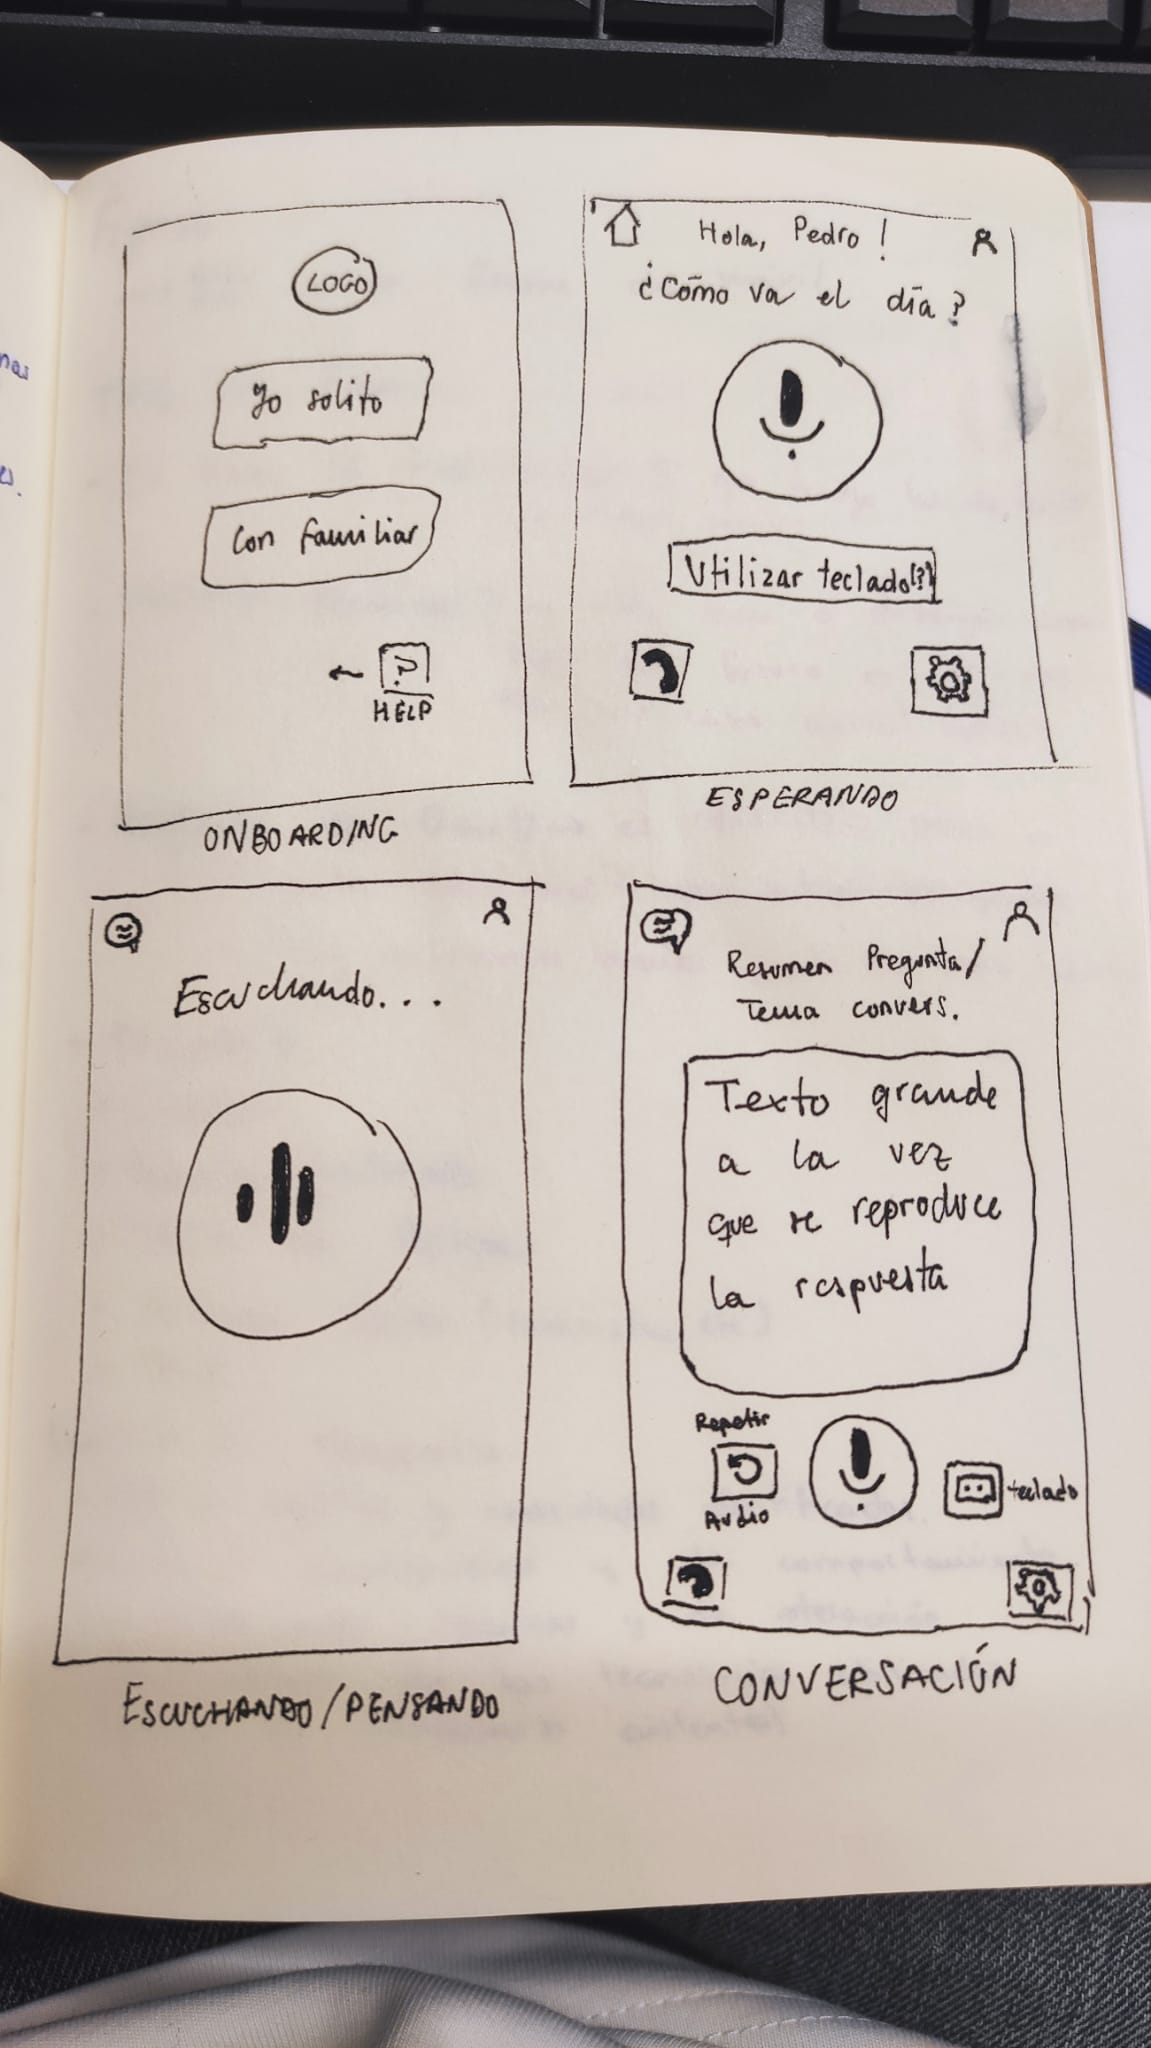
\includegraphics[height=11.5cm, trim={100 160 40 140}, clip]{imagenes/bocetos/boceto_mano_generico.jpeg}
  \caption[Bocetos a mano de los cuatro estados de la interfaz del mayor]{Bocetos iniciales a mano de los
  cuatro estados de la interfaz del mayor: selección de autonomía, espera, escucha y conversación.}
  \label{fig:boceto-libreta}
\end{figure}

\subsection{Wireframes en iPad}

La segunda etapa trasladó los bocetos supervivientes a wireframes digitales a escala, dibujados en iPad, y
su ganancia fue la \textbf{proporción}: es aquí donde las restricciones de accesibilidad dejaron de ser un
número en un documento de requisitos para convertirse en una limitación de espacio. Un botón de 88~px de
alto y un cuerpo de texto de 24~sp consumen enseguida la pantalla de un teléfono de gama media, y es el
wireframe el que hace evidente que no caben seis opciones y obliga a decidir cuáles son las dos que
importan.

% **note:** pendiente la exportacion de los wireframes de iPad. Cuando este disponible, colocar el fichero
% en imagenes/bocetos/ y descomentar el bloque siguiente (la figura no se referencia desde el texto, por eso
% se puede mantener comentada sin romper ninguna referencia).
%\begin{figure}[htbp]\centering
%  \includegraphics[width=0.9\textwidth]{imagenes/bocetos/wireframes-ipad.png}
%  \caption{Wireframes en iPad del flujo de \emph{onboarding} y de la pantalla principal.}
%  \label{fig:wireframes-ipad}
%\end{figure}

\subsection{Mockups con Claude Design}

La tercera etapa produjo \emph{mockups} de alta fidelidad con Claude Design, ya con color, tipografía y
jerarquía definitivos. Es la primera representación sobre la que se pueden tomar decisiones de paleta con
fundamento (y de hecho es donde se decidió sustituir el teal azulado inicial por la gama cálida justificada en el apartado~\ref{sec:color}) porque es la primera en la que el color aparece en su proporción
real y no como una muestra aislada.

\begin{figure}[htbp]\centering
  \begin{subfigure}[b]{0.46\textwidth}\centering
    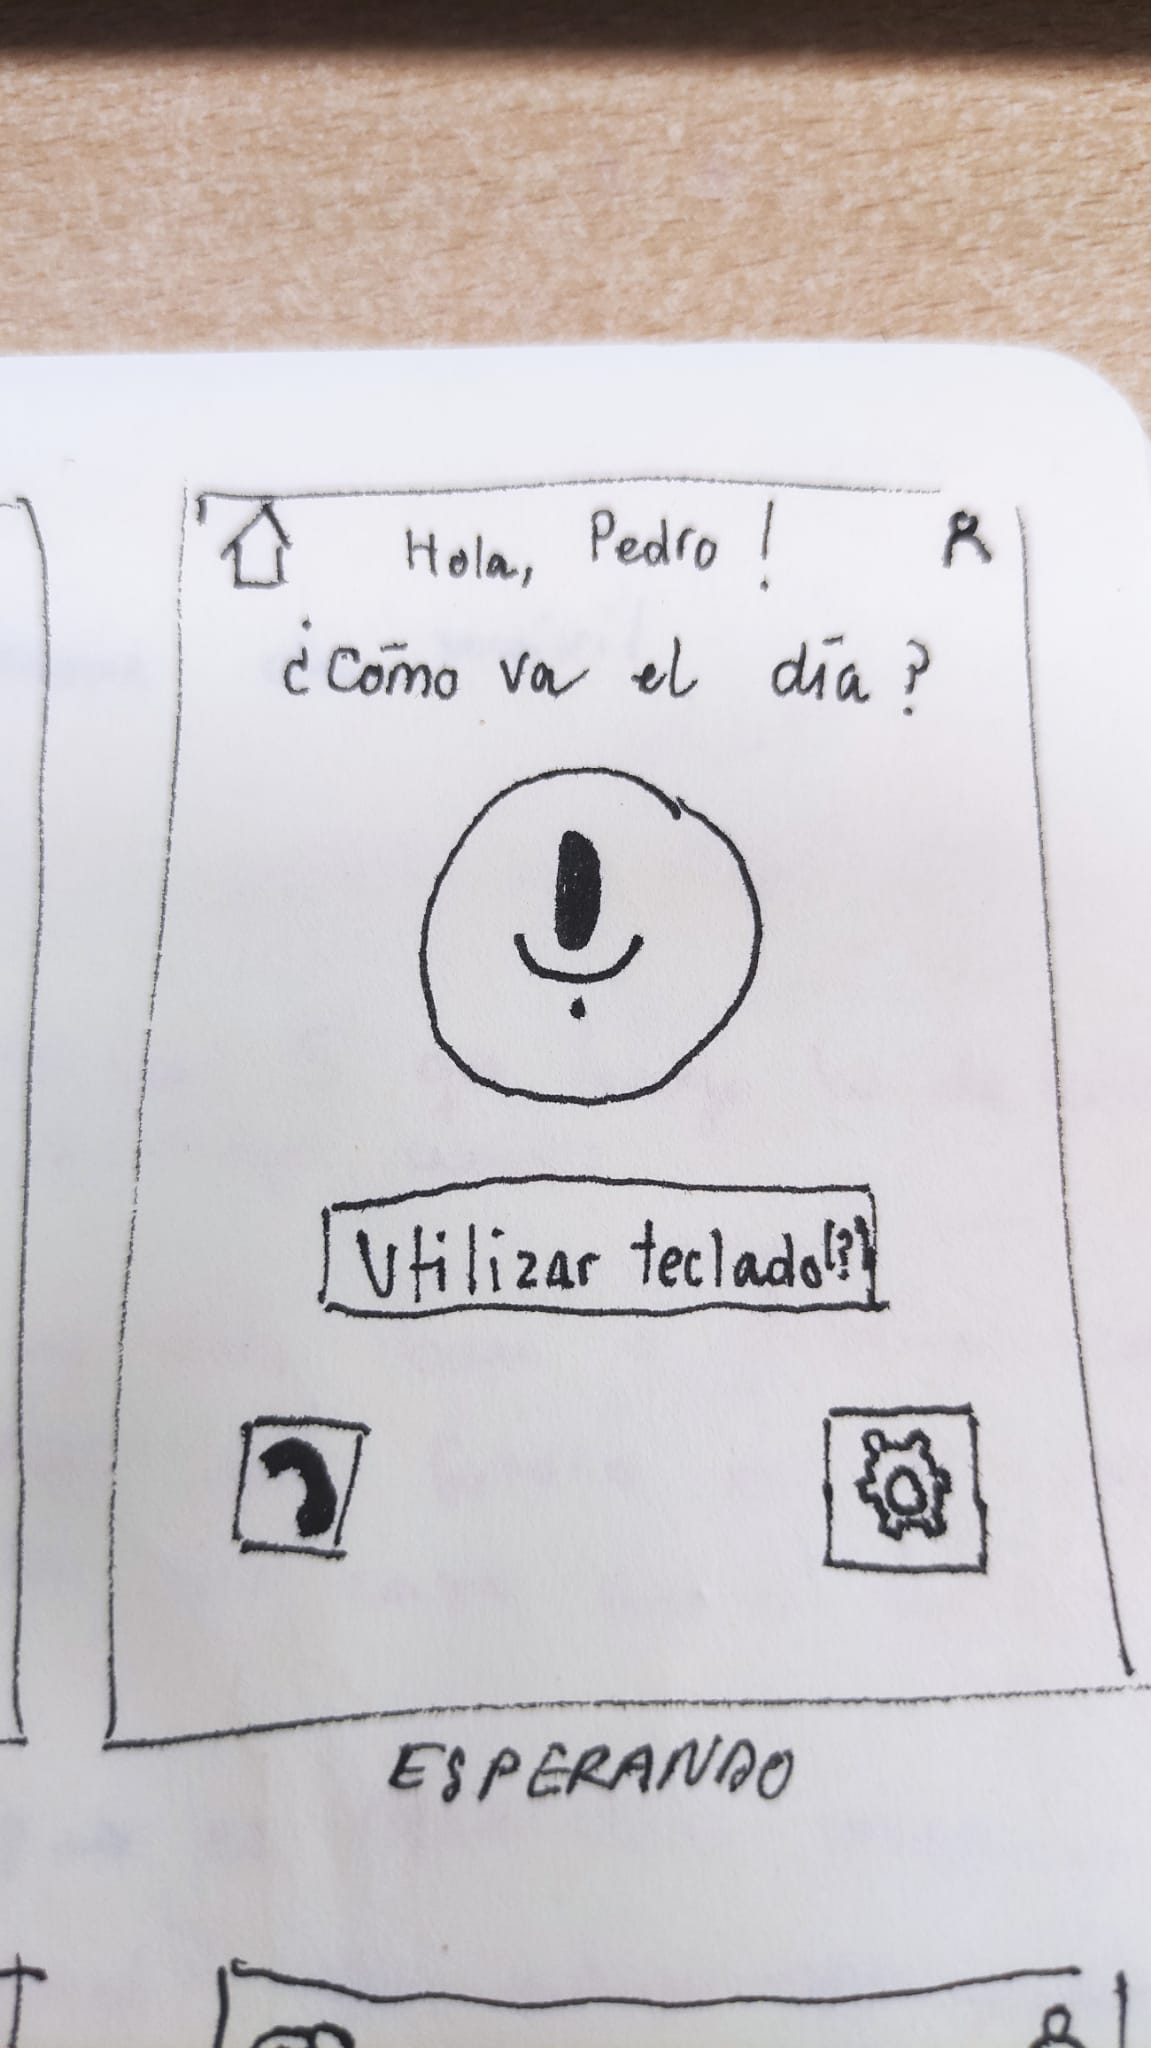
\includegraphics[height=9cm, trim={150 205 20 410}, clip]{imagenes/bocetos/boceto_mano_esp.jpeg}
    \caption{Boceto a mano}
  \end{subfigure}\hfill
  \begin{subfigure}[b]{0.46\textwidth}\centering
    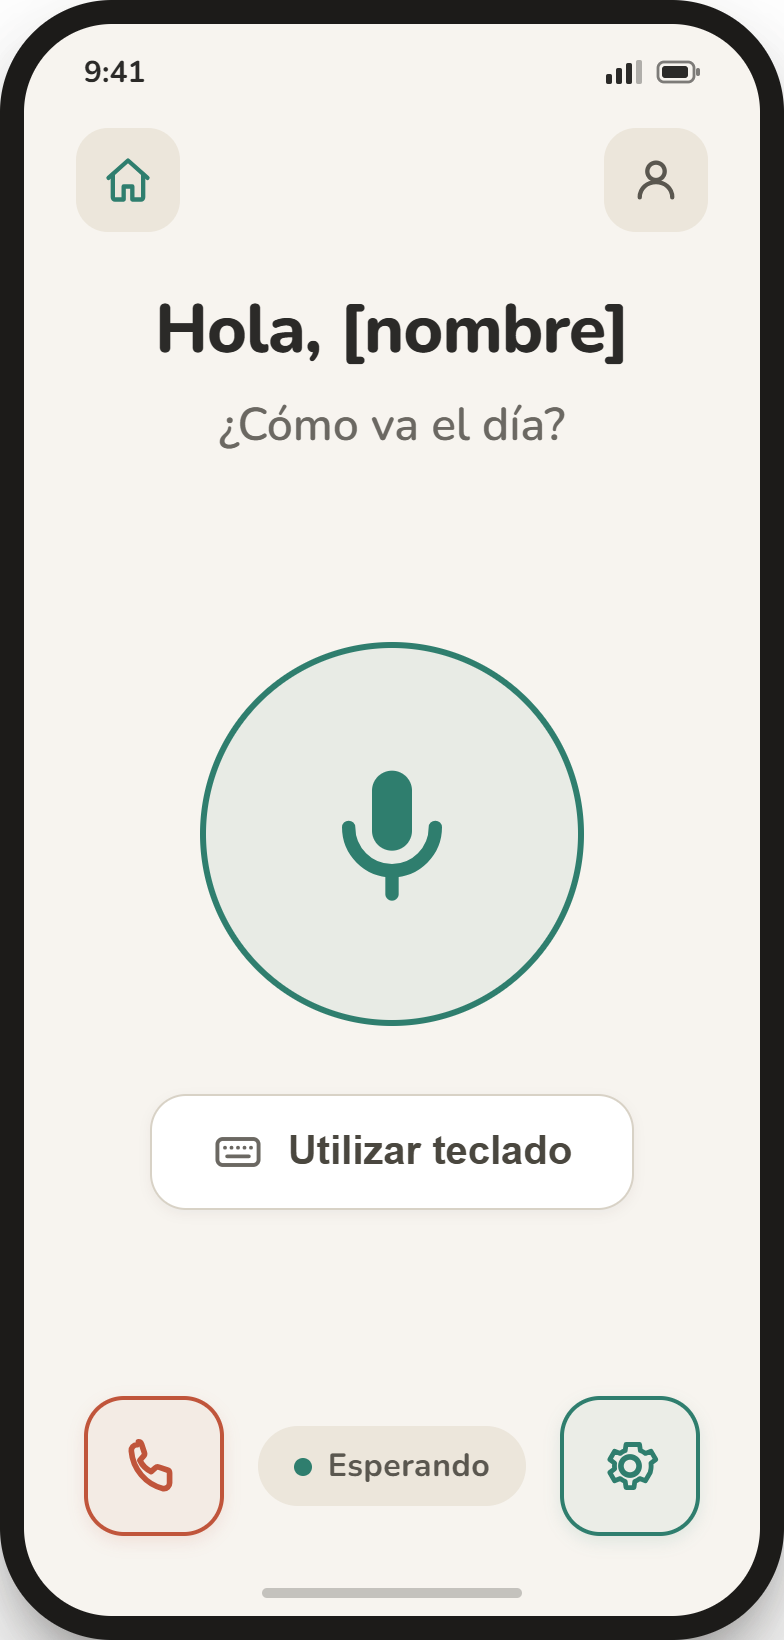
\includegraphics[height=9cm]{imagenes/bocetos/boceto_claude_design.png}
    \caption{\emph{Mockup} de alta fidelidad}
  \end{subfigure}
  \caption[Del boceto al \emph{mockup}: el estado de espera]{Del boceto al \emph{mockup}. La misma pantalla,
  el estado de espera, en la primera y en la tercera etapa de fidelidad. Se conservan la posición y el peso
  relativo de todos los elementos; lo que añade el \emph{mockup} es el color, la tipografía y la proporción
  real.}
  \label{fig:mockups}
\end{figure}

\subsection{Del mockup a Flutter: por qué se acortó la distancia diseño-código}

Los \emph{mockups} de esta etapa se trasladaron a Flutter con menos reinterpretación que las anteriores, y
el motivo es estructural y no de calidad gráfica. Un \emph{mockup} tradicional es una imagen a partir de la
cual el desarrollador reconstruye por su cuenta la jerarquía de contenedores; éstos llegaron descritos como
marcado con estilos, con una \textbf{jerarquía de composición ya explícita} que es isomorfa al árbol de
widgets: un contenedor en columna con separación uniforme es una \code{Column} con \code{spacing}, y una
caja con relleno y esquinas redondeadas, un \code{Container}. Lo que se acorta es el paso de \emph{inferir}
la estructura a partir de un dibujo, que es donde se introducen las divergencias entre lo diseñado y lo
construido. La ventaja se limita, eso sí, a la composición estática: el estado, la animación y el
comportamiento reactivo, donde reside la complejidad real de la pantalla principal, siguieron exigiendo el
trabajo de siempre.

\partesep{Parte II: Desarrollo}

\section{Stack tecnológico en uso}
\label{sec:stack}

Esta sección enuncia el \emph{stack} y cómo encajan sus piezas. La justificación de cada elección se
desarrolla en el apartado~\ref{sec:adr}, y las versiones son las fijadas en \code{pubspec.yaml}, verificadas
sobre el árbol de código.

El sistema es una \textbf{aplicación cliente Flutter} (Dart, SDK $\wedge$3.7.2) compilada para Android
(\code{minSdk} 24, \code{compileSdk} 36) apoyada en \textbf{Firebase} como \emph{Backend-as-a-Service}, en
un conjunto de \textbf{funciones propias desplegadas en Cloud Functions} y en dos servicios de Google Cloud
consumidos como API: Gemini, para la conversación y para el análisis de cada conversación al cerrarse, y
Cloud Text-to-Speech, para la voz.

\begin{table}[htbp]
    \centering
    \begin{tabularx}{\textwidth}{@{}l l >{\RaggedRight\arraybackslash}X@{}}
        \toprule
        \textbf{Capa} & \textbf{Componente} & \textbf{Función en el sistema} \\
        \midrule
        Cliente     & Flutter / Dart               & Interfaz nativa Android; sistema de diseño accesible propio \\
                    & \texttt{flutter\_riverpod} 2.5.1 & Estado reactivo e inyección de dependencias \\
                    & \texttt{go\_router} 17.0.0   & Enrutado declarativo con \emph{redirects} reactivos \\
                    & \texttt{speech\_to\_text} 7.3.0 & Transcripción de voz a texto (es-ES) \\
                    & \texttt{flutter\_tts} 4.2.5  & Síntesis de voz del dispositivo (hoy, respaldo) \\
                    & \texttt{just\_audio} 0.10.6  & Reproducción del audio sintetizado en la nube \\
                    & \texttt{url\_launcher} 6.3.2 & Apertura del marcador del sistema (emergencia) \\
                    & \texttt{permission\_handler} 12.0.1 & Permiso de micrófono \\
                    & \texttt{flutter\_dotenv} 6.0.0 & Carga de la clave de Gemini en desarrollo \\
        \midrule
        Backend     & \texttt{firebase\_core} 3.15.2 & Inicialización del SDK \\
                    & \texttt{firebase\_auth} 5.7.0  & Autenticación dual (anónima / correo) \\
                    & \texttt{cloud\_firestore} 5.6.0 & Persistencia y sincronización en tiempo real \\
                    & \texttt{cloud\_functions} 5.4.0 & Cliente de las cuatro \emph{callables} \\
                    & Cloud Functions (Node 22, gen 2) & Lógica de servidor (\autoref{tab:callables}) \\
        \midrule
        Servicios   & \texttt{google\_generative\_ai} 0.4.7 & Gemini \texttt{gemini-2.5-flash} en la conversación en vivo \\
                    & Vertex AI (\texttt{@google/genai}) & El mismo modelo en el servidor: análisis y memoria \\
                    & Cloud Text-to-Speech           & Voz \texttt{es-ES-Chirp3-HD-Sulafat} \\
        \bottomrule
    \end{tabularx}
    \caption{Stack tecnológico en uso, con las versiones fijadas en \texttt{pubspec.yaml} y en el
    \texttt{package.json} de las funciones.}
    \label{tab:stack}
\end{table}

Dos fijaciones de versión son deliberadas, aunque un lector técnico podría tomarlas por descuido:
\code{flutter\_riverpod} se mantiene en la línea 2.x por un conflicto de la 3.x con \code{scheduleNewFrame}
en el entorno de desarrollo Linux empleado, y todo el ecosistema FlutterFire se alinea sobre
\code{firebase\_core} 3.x para evitar conflictos de dependencias transitivas (ADR-0011). Ambas persiguen la
reproducibilidad del \emph{build} durante la evaluación del proyecto.

\section{Arquitectura realizada}
\label{sec:arquitectura}

Esta sección describe la arquitectura \textbf{tal como está construida}. Cuando la realización diverge del
modelo ideal, se indica.

\subsection{Visión general del sistema}
\label{sec:arquitectura-general}

Antes de entrar en la organización interna del código conviene situar las piezas que intervienen y cómo se
comunican entre sí, porque el sistema dejó de ser una aplicación aislada en el momento en que adquirió
servidor propio. La \autoref{fig:arquitectura} recoge esa visión de conjunto.

El sistema se despliega sobre \textbf{dos instancias del mismo binario}: la que ejecuta la persona mayor y
la que ejecuta el familiar. No son dos aplicaciones distintas, sino la misma, que se comporta de una u otra
forma en función del rol almacenado en el perfil, según el principio de revelación progresiva ya descrito.
Ambas se autentican contra \textbf{Firebase Authentication}, de forma anónima en el caso del mayor y con
correo y contraseña en el del familiar, y ambas observan la colección \code{users} de \textbf{Cloud
Firestore}, que actúa como memoria compartida entre los dos dispositivos y como mecanismo de propagación en
tiempo real de las preferencias.

El ciclo conversacional atraviesa cuatro piezas. La transcripción de la voz se resuelve \textbf{en el propio
dispositivo}, mediante el reconocedor del sistema operativo Android, de modo que el audio del mayor no sale
del terminal. El texto transcrito viaja a la \textbf{API de Gemini}, que devuelve la respuesta y que puede
además solicitar la ejecución de una función declarada por el cliente para guardar el nombre del mayor. Esa
respuesta se trocea en frases y cada una se envía a la \emph{callable} \code{synthesizeSpeech}, desplegada
en \textbf{Cloud Functions} sobre la región \code{europe-west1}, que a su vez invoca la \textbf{API de Cloud
Text-to-Speech} con una voz fija de servidor y devuelve el audio codificado. El reproductor del cliente lo
reproduce aplicando el volumen y la velocidad que el usuario tenga configurados y, si la síntesis en la nube
falla o agota su tiempo límite, la frase se pronuncia con el motor de voz del propio dispositivo. Cuando el
mayor prefiere escribir, el texto tecleado ocupa el lugar de la transcripción y la cadena es la misma, salvo
que la respuesta solo se sintetiza si él lo pide (apartado~\ref{sec:teclado}).

Tres caminos más atraviesan el servidor propio. El \textbf{emparejamiento} no se resuelve contra Firestore
desde el cliente, sino a través de la \emph{callable} \code{validateAndLink}, que localiza al mayor por su
código con credenciales de administrador y actualiza ambos perfiles en una única transacción. El
\textbf{consentimiento} del mayor sobre sus conversaciones solo puede escribirse a través de
\code{setConversationConsent}. Y al \textbf{cerrarse cada conversación}, el cliente entrega lo hablado a
\code{closeConversation}, que lo analiza con Gemini a través de Vertex AI, guarda únicamente el resultado y
descarta el texto; ese resultado llega después a los dos dispositivos por Firestore, como cualquier otro
dato. La \textbf{llamada de emergencia}, en cambio, no atraviesa el \emph{backend} en absoluto: construye un
URI \code{tel:} y cede el control al marcador del sistema operativo. Cerrando el conjunto, las \textbf{reglas
de seguridad de Firestore} se interponen en todo acceso de cliente a la base de datos, de manera que ni
siquiera un binario modificado puede leer o escribir fuera de lo que esas reglas permiten.

\begin{figure}[htbp]\centering
  %\includegraphics[width=\textwidth]{imagenes/arquitectura/arquitectura-sistema.png}
  \caption{Arquitectura del sistema: dispositivos, servicios gestionados y flujos de datos.}
  \label{fig:arquitectura}

  \vspace{2pt}
  {\footnotesize Fuente: Elaboración propia.}
\end{figure}
% **note:** añadir imagen del diagrama de arquitectura (mejor en PDF vectorial:
% imagenes/arquitectura/arquitectura-sistema.pdf) y descomentar el \includegraphics. Debe mostrar: los dos
% móviles (mayor y familiar) con el reconocimiento de voz en el dispositivo; Firebase Authentication;
% Firestore (users y las subcolecciones conversations, conversationContents y memory, con las reglas y la
% caducidad TTL); Cloud Functions en europe-west1 con las cuatro callables; Vertex AI (Gemini para el
% análisis); la API de Gemini llamada desde el cliente (conversación en vivo); Cloud Text-to-Speech; y el
% marcador tel: del sistema para la emergencia.

Merece la pena señalar una asimetría que el diagrama hace evidente y que el código no siempre deja ver: el
\emph{backend} propio interviene en la voz, el emparejamiento, el consentimiento y el análisis, pero
\textbf{no} en la conversación en vivo con el modelo de lenguaje, que el cliente sigue invocando directamente
con su propia clave. Ésa es la parte de ADR-0014 que queda por construir, y la razón por la que RNF-8 se
cumple solo a medias, según se detalla más adelante en este mismo capítulo.

\subsection{El servidor como plataforma gestionada: Firebase y Cloud Functions}
\label{sec:paas}

Que el sistema tenga servidor propio no significa que el proyecto opere un servidor. La distinción importa,
porque es la que hace viable un \emph{backend} con lógica propia para un único desarrollador, y se entiende
mejor con los modelos de servicio de la computación en la nube. El NIST define la plataforma como servicio
(PaaS) como la capacidad de desplegar en la infraestructura del proveedor aplicaciones propias, escritas con
los lenguajes y herramientas que éste admite, sin gestionar ni controlar la red, los servidores, el sistema
operativo ni el almacenamiento subyacentes: el cliente controla solo la aplicación desplegada y, en su caso,
la configuración del entorno que la aloja \citep{NIST800145}. Quiet Companion combina dos variantes de ese
modelo. Firebase actúa como \emph{Backend-as-a-Service} (ADR-0003): la autenticación y la base de datos se
consumen ya construidas, a través del SDK del cliente. Cloud Functions es una plataforma de funciones
(\emph{Function-as-a-Service}), la forma más acotada de PaaS, en la que la unidad de despliegue es una
función que el proveedor ejecuta bajo demanda, escala desde cero instancias y factura por invocación, de modo
que el desarrollador no administra máquina alguna \citep{Jonas2019}. En la segunda generación, que es la que
usa el proyecto, cada función se construye con Cloud Build y se despliega como un servicio de Cloud Run
\citep{FirebaseFunctionsVersions}.

Un BaaS basta mientras toda la lógica pueda vivir en el cliente, y el proyecto encontró tres cosas que un
cliente no puede hacer por sí solo. La primera es \textbf{guardar un secreto}: cualquier credencial
empaquetada en la aplicación puede extraerse del binario, y la síntesis de voz y el análisis necesitan
credenciales de Google Cloud (RNF-8). La segunda es \textbf{actuar sobre datos ajenos sin abrirlos a todos}:
las reglas de Firestore autorizan operaciones enteras y no ven las cláusulas de una consulta, de modo que lo
que exige buscar o escribir fuera del documento propio, como la vinculación, solo es seguro con privilegios
de servidor (RNF-9). La tercera es \textbf{dar fe}: la hora de un consentimiento, la comprobación de que
existe antes de analizar nada o el tope del plazo de conservación no pueden depender de lo que declare un
dispositivo que controla el propio usuario. Cada una de esas necesidades se tradujo en una función, y la
\autoref{tab:callables} recoge las cuatro que componen hoy el \emph{backend}.

\begin{table}[htbp]
    \centering
    \small
    \begin{tabularx}{\textwidth}{@{}l c >{\RaggedRight\arraybackslash}X >{\RaggedRight\arraybackslash}X@{}}
        \toprule
        \textbf{Función} & \textbf{ADR} & \textbf{Qué hace} & \textbf{Por qué en el servidor} \\
        \midrule
        \texttt{synthesizeSpeech}       & 0017, 0018 & Convierte una frase en audio con la voz Chirp~3:~HD
            & Las credenciales de Cloud TTS no salen del servidor, que fija además la voz \\
        \addlinespace
        \texttt{validateAndLink}        & 0024 & Vincula mayor y familiar por el código, en una transacción
            & Busca por código con privilegios de administrador sin que \texttt{/users} sea enumerable \\
        \addlinespace
        \texttt{setConversationConsent} & 0030 & Registra o retira el consentimiento del mayor
            & La hora del servidor es la prueba; programa el borrado de lo guardado \\
        \addlinespace
        \texttt{closeConversation}      & 0029, 0032 & Analiza la conversación al cerrarse y actualiza la
            memoria & Gemini sin clave; la transcripción no se almacena; aplica los plazos \\
        \bottomrule
    \end{tabularx}
    \caption{Funciones del \emph{backend}, todas \emph{callables} desplegadas en \texttt{europe-west1}.}
    \label{tab:callables}
\end{table}

Las cuatro comparten un mismo diseño, y son sus decisiones las que convierten la plataforma en una pieza
fiable. Todas son \emph{callables} (\code{onCall}) y no funciones HTTP genéricas ni disparadores de base de
datos: el SDK de Firebase adjunta y verifica el token de sesión en cada invocación, de modo que el servidor
toma la identidad de quien llama de \code{request.auth} y nunca de un parámetro, y nadie puede pedir que se
actúe en nombre de otro. Los disparadores se descartaron expresamente para el análisis, porque habrían
exigido escribir antes la transcripción en Firestore (ADR-0029). Todas se despliegan en \code{europe-west1},
junto a los datos, con un tope de diez instancias como salvaguarda de coste en un proyecto sin financiación,
y ninguna maneja claves: se autentican ante Cloud Text-to-Speech y Vertex AI con las credenciales por
defecto de la cuenta de servicio del entorno. La lógica con criterio, esto es, validar la entrada, sanear la
respuesta del modelo, aplicar los cambios de memoria o calcular cuándo caduca un dato, vive en módulos puros
separados de los manejadores, lo que permite probarla con \code{node --test} sin emulador ni red, en
cuarenta y cuatro casos. Y los registros siguen una regla sin excepciones: contienen longitudes e
identificadores, nunca texto de una conversación.

El beneficio más tangible de la plataforma no es técnico sino de proceso. Un cambio en el \emph{prompt} del
análisis o en la voz se publica con \code{firebase deploy}, sin generar ni instalar una APK nueva, y cada
análisis guarda la versión del \emph{prompt} que lo produjo. Los costes también existen y se aceptan con
conocimiento de causa: la primera invocación tras un periodo sin uso paga el arranque en frío de la
instancia, que en la voz cubre el respaldo al motor del dispositivo; la región debe coincidir en cliente y
servidor, porque el SDK apunta por omisión a \code{us-central1} y el desajuste no produce un error visible
(ADR-0018); y el proyecto queda ligado a la plataforma de Google, dependencia ya asumida al elegir Firebase.

\subsection{Estructura core/ y features/, y capas por \emph{slice}}

El código se organiza según el modelo híbrido Clean Feature-Sliced (CFS) prescrito por RNF-11: rebanadas
verticales de funcionalidad sobre un núcleo transversal.

\begin{lstlisting}[style=Consola, caption={Estructura real del árbol de código fuente.}, label={lst:arbol}]
lib/
|-- core/                 # lo que comparten dos o mas features
|   |-- config/           # router, redirect, filas de ajustes, plazos
|   |-- constants/        # firestore_paths
|   |-- models/           # usuario, consentimiento, conversacion...
|   |-- providers/        # currentUserProvider, linkedElderProvider...
|   |-- repositories/     # lectura de conversaciones y memoria
|   |-- services/         # Gemini, voz (STT y TTS), cierre...
|   |-- theme/            # AppTheme
|   |-- utils/            # sentence_splitter, week_summary
|   `-- widgets/          # ElderButton, SignOutButton
|-- features/
|   |-- conversation/  {data, domain, presentation}
|   |-- dashboard/     {domain, presentation}
|   |-- emergency/     {presentation}
|   |-- my_week/       {domain, presentation}
|   |-- onboarding/    {data, domain, presentation}
|   |-- privacy/       {data, domain, presentation}
|   `-- settings/      {presentation}
`-- main.dart, firebase_options.dart
functions/                # index.js (4 callables) y logica pura
firestore.rules, firestore-tests/
\end{lstlisting}

La regla que estructura el conjunto es la \textbf{ausencia de acoplamiento horizontal}: una \emph{feature}
no importa nunca de otra \emph{feature}; lo compartido asciende a \code{core/}. La regla no es
aspiracional, se ha hecho cumplir con coste: durante la estabilización se detectó que el \emph{dashboard}
importaba de \code{onboarding} y se rompió esa dependencia haciendo que el \emph{dashboard} leyera el
identificador del mayor vinculado del proveedor global en lugar del controlador ajeno.

Un ejemplo instructivo de la regla en acción es \code{settings\_rows.dart}. Las filas de la pantalla de
ajustes viven en \code{core/config/} y no en \code{features/settings/}, aunque intuitivamente pertenezcan
a esa \emph{feature}, porque las consumen dos \emph{features} que no pueden acoplarse entre sí:
\code{conversation} decide con ellas si muestra el botón de Ajustes, y \code{settings} decide qué
renderiza. Ubicar la lista en cualquiera de las dos habría obligado a la otra a importarla. La misma regla
gobernó los incrementos posteriores al MVP: la agregación semanal que muestran el panel del familiar y
«Mi semana» vive en \code{core/utils/week\_summary.dart}, y los modelos y repositorios de lectura del
análisis en \code{core/}, porque los consumen dos \emph{features} que tampoco pueden importarse entre sí.

La estructura por capas no es uniforme entre \emph{slices}, y esto es intencionado: \code{emergency} y
\code{settings} tienen solo \code{presentation} porque su lógica se resuelve con servicios de \code{core/}
y funciones puras, sin estado propio. Crear una carpeta \code{domain} vacía por simetría sería el tipo de
sobreingeniería que la propia investigación arquitectónica del proyecto advertía evitar.

La regla tiene una deuda conocida: \code{authRepositoryProvider} y \code{SignOutButton} nacieron en
\code{onboarding} y se promovieron a \code{core/} cuando otras \emph{features} los necesitaron, lo que
difumina en esos dos puntos la frontera entre núcleo y \emph{feature}.

\subsection{Single Source of Truth: \texttt{currentUserProvider}}
\label{sec:ssot}

Varias partes del sistema necesitan el documento \code{users/\{uid\}} en tiempo real: el enrutador para
decidir redirecciones, la pantalla principal para el tamaño de letra, el servicio de voz para el volumen y
la velocidad, y el panel del familiar. Que cada uno abriese su propia suscripción a Firestore duplicaría
escuchas y repartiría la responsabilidad de mantener el dato.

La arquitectura adopta un \textbf{único punto de escucha} (ADR-0009). \code{firebaseAuthUserProvider} emite
el usuario de Firebase Auth; \code{currentUserProvider} lo observa y, cuando hay sesión, se suscribe a
\code{users/\{uid\}} y lo mapea a \code{UserModel}. Cualquier widget o controlador, en cualquier punto de
la aplicación, se limita a observar ese proveedor con \code{ref.watch}, y Riverpod reconstruye solo a los
observadores efectivos cuando Firestore emite.

La consecuencia observable de este diseño es la propiedad más vistosa del sistema. Cuando el familiar
completa el emparejamiento, la transacción borra el \code{linkCode} del documento del mayor; el
\emph{stream} emite, el enrutador recalcula su decisión y \textbf{el dispositivo del mayor navega solo a la
pantalla principal}, sin que el mayor pulse nada. El mismo mecanismo, sin código adicional, es el que
propaga en caliente las preferencias de accesibilidad (RF-6).

Esta decisión implicó retrabajo real: \code{ElderAuthController} mantenía su propia suscripción al mismo
documento, en paralelo al proveedor, y el enrutador decidía con datos obsoletos del controlador. La
suscripción se eliminó en la estabilización, aunque sobrevive un camino redundante (\code{checkPairingStatus()}
y su botón «Continuar») marcado en el código para eliminación.

El patrón tuvo que extenderse después al lado del familiar, y el motivo es instructivo (ADR-0027). El panel
leía el documento del mayor una sola vez al abrirse, y cada deslizador reescribía después el documento
entero a partir de esa copia. Mientras el familiar era el único que escribía, la copia no envejecía; desde
que el mayor ajusta sus propias escalas y el asistente aprende su nombre, el siguiente deslizador del
familiar revertía esos cambios en silencio o fallaba contra las reglas. La corrección aplica a las
escrituras la misma lección que ADR-0009 aplicó a las lecturas: \code{linkedElderProvider} es para el
familiar lo que \code{currentUserProvider} es para el propio usuario, el panel pinta desde ese \emph{stream}
y cada control escribe solo su campo, con una ruta de punto (\code{preferences.volume}), de modo que dos
escrituras sobre magnitudes distintas ya no se pisan. Fue además el requisito previo de todo lo que vino
después: sin él, cada campo nuevo del documento del mayor habría sido una fuente más de errores al
guardar.

\subsection{Gestión de estado e inyección de dependencias}

Todo estado de negocio se modela como un \code{StateNotifier} sobre una clase de estado inmutable con
\code{copyWith}. No se usa \code{setState} para lógica de negocio en ningún punto; las pantallas son
\code{ConsumerWidget} o \code{ConsumerStatefulWidget} que observan y renderizan. El único estado local
admitido en la capa de presentación es el estrictamente efímero de un widget: la posición de un
deslizador mientras se arrastra, la posición de un \code{ScrollController}.

Riverpod cubre simultáneamente el estado reactivo y la inyección de dependencias (RNF-12): servicios y
repositorios se resuelven vía \code{Provider} y se pasan por constructor, nunca se instancian dentro de la
clase que los usa. Esto es lo que hace testable el sistema sin dobles de plataforma: los tests de la
pantalla de emergencia sustituyen \code{TtsService}, \code{SpeechService} y \code{EmergencyCallService} por
falsos sin tocar los \emph{plugins} reales.

Este cumplimiento no fue de partida: una revisión de arquitectura a mitad de HU-4 detectó que
\code{GeminiService} y \code{SpeechService} se instanciaban dentro del proveedor del \code{ChatController},
y se corrigió en ese momento; hoy el controlador recibe todos sus servicios por constructor.
% **note:** CLAUDE.md sigue listando `new GeminiService()` en chat_controller.dart:86 como deuda técnica
% pendiente; esa entrada está obsoleta (la migración a DI está hecha). Lo mismo con las advertencias de
% `withOpacity` y los `print()` de home_screen.dart, que ya no existen en el árbol.

\subsection{Operaciones atómicas y enrutado reactivo}

El emparejamiento entre mayor y familiar exige modificar \textbf{dos documentos} de usuarios distintos sin
que pueda quedar un estado intermedio en el que uno esté vinculado y el otro no. Se resuelve con una
transacción de Firestore que revalida el código dentro de ella y actualiza ambos documentos en una sola
operación. La transacción sustituyó en su día a un lote de escritura (\code{WriteBatch}) por una razón
concreta: un lote no puede \emph{leer}, y la desnormalización del contacto de emergencia exige leer antes el
documento del mayor para respetar la precedencia de un contacto fijado manualmente sobre el heredado del
familiar. Hoy esa transacción no se ejecuta en el cliente sino dentro de \code{validateAndLink}; el
apartado~\ref{sec:adr-identidad} cuenta por qué tuvo que moverse.

El enrutado es reactivo. \code{RouterNotifier} observa los dos controladores de autenticación, el estado de
Firebase Auth y \code{currentUserProvider}, y notifica a \code{go\_router} en cada cambio para que
recalcule la redirección. La decisión de destino se toma sobre el dato en vivo del proveedor, con el estado
del controlador únicamente como respaldo durante el intervalo previo a la primera emisión del \emph{stream},
y una guarda de rol impide que el documento de un familiar se use para decidir la ruta de un mayor. Esa
decisión vive en una función pura, \code{routeRedirect}, extraída para que las pruebas del enrutador
ejerciten la lógica real y no una copia escrita a mano. Ahí se implementa también la pregunta del
consentimiento: un mayor ya dado de alta que nunca ha respondido es dirigido a \code{/consent} antes de
llegar a la pantalla principal (apartado~\ref{sec:privacidad}).

\section{Decisiones de arquitectura y desarrollo}
\label{sec:adr}

Durante el proyecto se registraron treinta y siete decisiones de arquitectura (ADR) con su contexto, sus
alternativas evaluadas y sus consecuencias. Esta sección expone por temas las que dieron forma al MVP; las
posteriores, que sostienen HU-5 a HU-8, se resumen al final y se desarrollan en los apartados que siguen.
La \autoref{tab:adr} las recoge todas con su estado de implementación verificado sobre el código.

\subsection{Plataforma, stack y dependencias}

El primer bloque fija el terreno de juego, y sus tres primeras decisiones se tomaron en la misma semana
porque están encadenadas.

La elección del \textbf{framework de cliente} (ADR-0001) descartó de inmediato el desarrollo nativo por
plataforma, que duplica el esfuerzo de un desarrollador único, y entre las opciones multiplataforma decidió
el \textbf{control de la interfaz}: la accesibilidad del proyecto exige redefinir por completo el sistema de
diseño, y Flutter lo permite sin depender de los componentes estándar del sistema operativo, mientras que
una aplicación web añadía un peor acceso al micrófono. El coste asumido es que iOS es una plataforma posible
pero \textbf{no verificada}.

La \textbf{inteligencia conversacional} (ADR-0002) se delega en un LLM en la nube, Gemini
\code{gemini-2.5-flash}: no tendría sentido elegir un framework por su alcance a terminales de gama
media-baja y exigir después a esos terminales inferencia neuronal local, y el \emph{fine-tuning} de un modelo
propio era inviable sin datos conversacionales. El tono empático se consigue mediante \emph{prompt
engineering}, con la instrucción de sistema y los filtros de seguridad configurados en \code{GeminiService}.
% **note:** la selección de Gemini frente a GPT-4o-mini o Claude Haiku está evidenciada por el código pero
% su justificación (capa gratuita, function calling, mismo proyecto GCP) no consta en la fuente documental;
% decidir si se redacta un ADR de selección de proveedor o basta con el párrafo anterior. Ver ADR-0002.

El \textbf{backend} (ADR-0003) es Firebase como \emph{Backend-as-a-Service}, descartando un servidor propio
tipo Spring Boot o Django que un desarrollador único con plazo fijo no podría construir y operar; prescindir
de \emph{backend} era imposible, porque mayor y familiar necesitan sincronizarse entre dispositivos.
Firestore, con sus \emph{streams} de documento, es además lo que hace viable la fuente única de verdad
(apartado~\ref{sec:ssot}), y el BaaS se completó después con funciones propias (apartado~\ref{sec:paas}).

La \textbf{gestión de estado} (ADR-0005) es la única decisión del bloque que contradice la investigación
previa del propio proyecto, que recomendaba BLoC con GetIt y fpdart: se optó por Riverpod porque un solo
mecanismo cubre estado e inyección y porque \code{StreamProvider} mapea de forma natural los
\emph{snapshots} de Firestore. La divergencia es consciente, y su coste, el anclaje en la línea 2.x, se ha
descrito en el apartado~\ref{sec:stack} junto a la alineación de dependencias de ADR-0011.

\subsection{Arquitectura y gestión de estado}

El \textbf{modelo arquitectónico} (ADR-0004) descartó la organización por capas técnicas, por su fricción al
escalar, la organización por \emph{features} pura, por carecer de reglas contra el acoplamiento lateral, y el
FSD estricto, por riesgo de sobreingeniería frente al plazo. El resultado toma la macroestructura de CFS con
la nomenclatura de Clean Architecture, que es la que un tribunal reconoce sin glosario. La \textbf{fuente
única de verdad} (ADR-0009) se ha descrito en el apartado~\ref{sec:ssot}.

La \textbf{persistencia de preferencias desde el panel del familiar} (ADR-0010) resuelve dos problemas en el
mismo camino de escritura. Uno de coste: un deslizador emite decenas de eventos por segundo, así que se
escribe en \code{onChangeEnd}, una vez por gesto. Otro de honestidad: la actualización es optimista pero con
\textbf{reversión real} si la escritura falla, en lugar de dejar en pantalla un valor que nunca llegó a
guardarse. ADR-0027 conservó esa garantía cambiando su mecanismo: con el panel suscrito en vivo, es la
propia caché de Firestore la que revierte el valor rechazado.

La \textbf{aplicación de las preferencias de voz} (ADR-0019) la provocó la migración de la síntesis a la
nube, cuyo diseño fijaba que el cliente enviara solo texto para reducir la superficie de abuso de la
función; aplicado al pie de la letra, los deslizadores de volumen y velocidad habrían dejado de tener
efecto. La solución las aplica en el \textbf{reproductor} del cliente: el servidor sintetiza a ritmo neutro y
el reproductor ajusta velocidad y volumen con el mismo factor de conversión que \code{flutter\_tts} aplica en
Android, de modo que el ajuste significa lo mismo con las dos voces.

\subsection{Identidad, roles y emparejamiento}
\label{sec:adr-identidad}

La \textbf{autenticación} (ADR-0006) es dual porque los dos actores tienen necesidades opuestas: el mayor
usa autenticación anónima ligada al dispositivo, porque exigirle correo y contraseña sería una barrera real,
y el familiar usa correo y contraseña porque necesita una cuenta portable. El corolario no es opcional:
\textbf{el mayor no tiene cierre de sesión}, porque cerrarla generaría un identificador nuevo y perdería su
perfil, y el coste asumido es que una reinstalación crea un usuario nuevo. La \textbf{revelación
progresiva} (ADR-0007) se ha tratado entre los principios de diseño.

La \textbf{configuración explícita de accesibilidad} (ADR-0013) rechaza deliberadamente la adaptación
automática por IA, que habría sido técnicamente sencilla: para este colectivo un cambio de interfaz no
solicitado desorienta, la inferencia es opaca y falible, y un error del sistema erosiona una confianza que
costó construir. La decisión estuvo mucho tiempo implementada a medias, porque solo existía la ruta remota
del familiar y el mayor no podía ajustar nada desde su propio dispositivo. Desde ADR-0021 existen las
\textbf{escalas locales} de tamaño de letra, volumen y velocidad de la voz, resueltas como peldaños con
nombre («Normal», «Grande», «Muy grande») en lugar de deslizadores, porque un deslizador exige una precisión
motora que esta población no tiene por qué tener y un valor sin nombre no le dice nada a quien lo elige.
Están disponibles para todo mayor, y con ellas CU-05 queda \textbf{cubierto}. ADR-0036 añadió después una
cuarta escala con el mismo patrón.

El \textbf{emparejamiento} fue durante cuatro meses la decisión más incómoda del proyecto, y su historia
completa, incluida la parte en que estuvo mal, es más instructiva que su estado final.

ADR-0008 lo implementó como una \textbf{transacción de cliente} que escribía en el documento del mayor
desde la sesión del familiar. Fue una decisión de desbloqueo consciente: sin infraestructura de servidor
desplegada en aquel momento, la alternativa era detener HU-1 a la espera de construirla. Se asumió como
provisional, con la reserva de seguridad anotada en el propio ADR y en el código, de modo que la deuda quedó
registrada antes de que nadie la cobrase.

La factura llegó al escribir las reglas de seguridad reales (ADR-0025), y fue más cara de lo anotado. La
reserva de ADR-0008 hablaba de una \emph{escritura} que las reglas denegarían; el problema mayor estaba en
la \emph{lectura}. Encontrar al mayor a partir de su código de cuatro caracteres es una consulta de
colección (\code{where('linkCode', '==', code)}), y \textbf{las reglas de Firestore no ven las cláusulas
de una consulta}: solo pueden permitir o denegar la operación entera. Mientras la búsqueda viviera en el
cliente, \code{/users} tenía que ser consultable por cualquier usuario autenticado; es decir, cualquiera con
la aplicación instalada y una sesión anónima podía enumerar el directorio de usuarios, con sus nombres y sus
teléfonos de contacto. La arquitectura provisional no incumplía un requisito en abstracto: dejaba una puerta
abierta que nadie había medido.

Medido el coste, la migración dejó de ser opcional. ADR-0024 traslada la vinculación a la \emph{callable}
\code{validateAndLink}, en el mismo \emph{codebase} de Cloud Functions que ya servía la síntesis de voz
(ADR-0018). El identificador del familiar deja de ser un parámetro y lo toma el servidor de la sesión
autenticada, de modo que nadie puede pedir que se vincule a un tercero; la búsqueda corre con credenciales
de administrador, lo que permite cerrar \code{allow list} sobre \code{/users}; el código se consume dentro
de la misma transacción que lo valida; y aparecen dos comprobaciones que el cliente no podía hacer sobre sí
mismo, entre ellas que quien vincula sea realmente un familiar registrado. \textbf{RNF-9 se cumple}, y
ADR-0008 queda formalmente superado por ADR-0024.

Conviene subrayar el orden de los acontecimientos, porque es el argumento de proceso y no de resultado:
\textbf{primero se escribieron las reglas, y fueron las reglas las que obligaron a mover el código}. Los
primeros veintinueve casos de prueba se redactaron incluyendo los huecos, casos que documentaban lo que las reglas todavía permitían, y fue eso lo que hizo visible el problema de la enumerabilidad. El test se
escribió antes que la solución y sirvió para encontrarla.

Las \textbf{reglas de seguridad} (ADR-0025) responden a una pregunta que no es obvia: si se modela el
sistema que se quiere o el que existe. Las anteriores describían la arquitectura pretendida, con una
colección que ningún código escribía, y enmascararon durante meses que el código las contradecía. Las
actuales modelan \textbf{operación por operación} lo que hace el código: lectura solo por identificador,
para el dueño y para el familiar vinculado; borrado siempre denegado; escritura del familiar acotada por
campo a las preferencias, el nombre y, desde ADR-0034, los plazos de la conversación, de modo que el panel
no puede cambiar el rol del mayor, romperle el vínculo, reescribirle el contacto de emergencia ni decidir
sobre su consentimiento; y denegación por defecto para todo lo demás. Se busca que las reglas \textbf{fallen
en voz alta}: si una operación cambia y las reglas no la contemplan, la aplicación muestra un error y las
pruebas lo señalan, en vez de quedar siendo falsas en silencio.

Su \textbf{verificación} (ADR-0026) es una decisión aparte porque las reglas son código con una
particularidad incómoda: cuando fallan no avisan al desarrollador, fallan en el dispositivo del usuario. Se
prueban contra el emulador de Firestore con casos agrupados por sujeto (el dueño, el familiar vinculado, un
autenticado cualquiera, un no autenticado), que eran veintinueve al cerrar el MVP y son cuarenta y ocho tras
incorporar el consentimiento y el análisis; el emulador exige un JDK~21 que convive con el del \emph{build}
de Android anteponiéndolo solo en el comando que lo necesita (ADR-0023). Es la única parte del proyecto
donde se verifica no que el sistema haga lo correcto, sino que \textbf{niegue lo incorrecto} a quien no es
el cliente de la aplicación.

\subsection{IA conversacional, voz y proxy seguro}

Este bloque contiene la única decisión de seguridad del proyecto todavía \textbf{no completada} y las
que resolvieron la calidad y el turno de la voz.

El \textbf{proxy de Cloud Functions para la clave del LLM} (ADR-0014) está \textbf{construido solo en
parte}, y conviene decirlo sin eufemismos porque la fuente documental del propio proyecto lo califica de
«requisito de seguridad crítico». Desde ADR-0029, el análisis de cada conversación al cerrarse llama a
Gemini desde el servidor, a través de Vertex AI y con las credenciales del entorno, sin clave alguna. La
conversación en vivo, en cambio, sigue partiendo del cliente: \code{GeminiService} obtiene la clave de
\code{Env.geminiApiKey}, que la lee del fichero \code{.env} empaquetado como recurso de la aplicación. Esa
clave, por tanto, \textbf{reside todavía en el cliente}, y RNF-8 solo se cumple en las funcionalidades que se
apoyan en el servidor. Lo que queda no es construir infraestructura, porque el \emph{codebase} de Cloud
Functions existe y sirve cuatro funciones, sino escribir una quinta que actúe de intermediaria en cada turno;
su coste es de latencia y de integración en el camino que más se usa, y por eso se aborda en el
\autoref{cap:desarrollo-futuro}. Tras el cierre de RNF-9, éste es el \textbf{único incumplimiento de
seguridad declarado} que le queda al proyecto.

La \textbf{sustitución del TTS del dispositivo por voz en la nube} (ADR-0017) es la decisión de producto
más visible. El motor nativo de Android produce una voz perceptiblemente robótica, cuya calidad depende
además del motor instalado en cada dispositivo, y para una población mayor una voz poco natural reduce la
inteligibilidad y la disposición a conversar. La elección recayó en Cloud Text-to-Speech con voces
Chirp~3:~HD en es-ES, tras descartar Azure, por introducir un segundo proveedor sin ganancia funcional,
ElevenLabs y OpenAI, por coste o por voces optimizadas para inglés, y los modelos abiertos en el
dispositivo, por reintroducir el problema de hardware que ADR-0002 evitó. Dos elementos merecen atención: el
\textbf{troceado por frases}, que sintetiza la primera oración y la reproduce mientras se sintetiza la
siguiente, de modo que el primer audio llega tras un solo viaje de red; y la \textbf{política de respaldo
sin reintentos}, que pronuncia con el motor del dispositivo cualquier frase cuya síntesis falle o tarde,
porque para este usuario una voz peor pero inmediata es preferible a un silencio imprevisible.

La \textbf{creación del codebase de Cloud Functions} (ADR-0018) documenta un descubrimiento de
implementación: el diseño de la migración situaba la nueva función «en el codebase existente», y ese
codebase \textbf{no existía}, porque ADR-0014 nunca había pasado de propuesta. Se creó con \textbf{una única
función}, \code{synthesizeSpeech}, sobre la segunda generación, Node~22 y la región \code{europe-west1}, y se
descartó migrar en el mismo movimiento la conversación en vivo, porque tocaba el camino más usado justo
antes de las pruebas. El \emph{codebase} que nació con una función sirve hoy cuatro
(\autoref{tab:callables}).

La \textbf{excepción de tráfico en claro hacia loopback} (ADR-0020) fue la consecuencia imprevista de la
anterior. En el primer despliegue real la síntesis funcionaba y el audio no sonaba: \code{just\_audio} sirve
los bytes desde un servidor HTTP local en \code{127.0.0.1}, y desde Android~9 el tráfico en claro está
prohibido por defecto, sin distinguir entre un servidor remoto y el del propio proceso. Se permitió ese
tráfico \textbf{exclusivamente} hacia loopback, descartando el atributo global que lo habría abierto a cualquier
destino. En la misma sesión apareció un segundo defecto, las respuestas de varias frases reproducían solo la
primera y la última, por una suposición equivocada sobre cuándo completa el método de reproducción del
\emph{plugin}. Ninguno de los dos era detectable por las pruebas, y no por falta de cobertura: el doble de
prueba cumplía por construcción el contrato que el \emph{plugin} real incumplía. En la costura con una
librería externa, la prueba protege del error propio, no de una suposición equivocada sobre la librería;
eso solo lo dice el dispositivo.

La \textbf{escucha por turnos} (ADR-0022) volvió a demostrarlo. El reconocedor nativo de Android corta su
sesión en cada pausa, de modo que la aplicación encadena sesiones y da el turno por terminado tras un
silencio, sin que el mayor tenga que pulsar nada. La primera prueba completa en dispositivo sacó a la luz
dos defectos que ninguna prueba automática podía ver (ADR-0036): la última palabra de cada frase se perdía,
porque el sistema avisa de que ha dejado de grabar antes de entregar el único resultado que la contiene, y
los dos segundos de silencio fijados en el código cortaban al mayor a media idea. El primero se corrigió
esperando a ese resultado final, con un tope de un segundo; el segundo dejó de ser una constante y pasó a
ser una escala más de Ajustes, «Tiempo que te espero», de dos a diez segundos y tres por omisión, porque
cuánto se detiene alguien a pensar depende de la persona.

\subsection{Acompañamiento, datos y privacidad}

La \textbf{llamada de emergencia} (ADR-0012) lanza el marcador del sistema con el número premarcado,
mediante un URI \code{tel:}, en lugar de marcar directamente desde la aplicación, lo que habría exigido el
permiso peligroso \code{CALL\_PHONE} y abierto la puerta a una llamada accidental al 112. El coste es un toque
adicional; el beneficio, un paso de confirmación en el punto exacto donde una equivocación es más cara.

Las dos decisiones restantes del bloque son de privacidad, y lo instructivo es cómo se cerraron. La
\textbf{persistencia conversacional} (ADR-0015) fijó el principio de guardar de cada conversación un resumen
junto a metadatos de sesión, nunca la transcripción cruda, y proponía generar ese resumen \textbf{en el
cliente}. La \textbf{salida de la transcripción al proveedor del LLM} (ADR-0016) fue su contrapartida
honesta y la única decisión registrada deliberadamente \textbf{sin cerrar}: no persistir no equivale a no
procesar, porque para resumir hay que enviar la transcripción al proveedor, y quedaba por decidir qué cubría
el consentimiento y quién lo otorgaba, si el mayor como titular del dato o el familiar como tercero.
Ninguna de las dos se implementó tal como estaba escrita. Al abordar HU-5 y HU-6, ADR-0029 conservó el
principio de ADR-0015 pero trasladó el análisis al servidor, y ADR-0030 respondió a la pregunta abierta de
ADR-0016; ambas se desarrollan en los apartados~\ref{sec:conversacion} y~\ref{sec:privacidad}.

\subsection{Decisiones posteriores al MVP}

Las decisiones que siguen al MVP dan forma a HU-5 a HU-8, y su peso en el resultado justifica tratarlas
aparte. ADR-0027 llevó al panel del familiar el patrón de fuente única de verdad y fue su requisito previo
(apartado~\ref{sec:ssot}). ADR-0028, ADR-0029, ADR-0032 y ADR-0033 definen qué es una conversación, cómo se
analiza al cerrarse, qué recuerda el asistente y cómo se presenta el resultado
(apartado~\ref{sec:conversacion}). ADR-0030, ADR-0031 y ADR-0034 construyen el consentimiento y el gobierno
de los datos (apartado~\ref{sec:privacidad}), y ADR-0035 añade la conversación por escrito
(apartado~\ref{sec:teclado}). ADR-0036, por último, corrige la escucha a partir de la primera prueba
completa en dispositivo, como se ha visto más arriba.

\subsection{Tabla resumen de decisiones}

La \autoref{tab:adr} recoge las treinta y siete decisiones con su alternativa principal descartada y su
estado de implementación. El estado se ha determinado \textbf{leyendo el código}, no la documentación de diseño:
«Implementado» significa que existe el código que sostiene la capacidad de extremo a extremo; «Parcial»,
que solo una parte del alcance decidido está construida; y «Superada» o «Cerrada», que una decisión
posterior la sustituyó o respondió a la cuestión que dejaba abierta.

\begin{longtable}{@{}l >{\RaggedRight\arraybackslash}p{0.30\textwidth} >{\RaggedRight\arraybackslash}p{0.30\textwidth} l@{}}
\caption{Resumen de las decisiones de arquitectura (ADR) y su estado de implementación verificado sobre el código.}
\label{tab:adr} \\
\toprule
\textbf{ID} & \textbf{Decisión} & \textbf{Alternativa descartada} & \textbf{Estado} \\
\midrule
\endfirsthead
\multicolumn{4}{c}{\tablename\ \thetable{} \textit{(continuación)}} \\
\toprule
\textbf{ID} & \textbf{Decisión} & \textbf{Alternativa descartada} & \textbf{Estado} \\
\midrule
\endhead
\midrule \multicolumn{4}{r}{\textit{continúa en la página siguiente}} \\
\endfoot
\bottomrule
\endlastfoot
0001 & Flutter multiplataforma            & Desarrollo nativo por plataforma        & Implementado \\
0002 & LLM conversacional en la nube      & Modelo abierto en el dispositivo        & Implementado \\
0003 & Firebase como BaaS                 & Servidor propio (Spring Boot / Django) & Implementado \\
0004 & Arquitectura Clean Feature-Sliced  & \emph{Layer-first} / FSD estricto       & Implementado \\
0005 & Riverpod (estado + DI)            & BLoC + GetIt + fpdart                   & Implementado \\
0006 & Auth dual anónima / correo         & Correo y contraseña para ambos roles    & Implementado \\
0007 & Revelación progresiva              & Dos flujos o dos aplicaciones           & Implementado \\
0008 & Emparejamiento por transacción de cliente & \emph{Cloud Function} \emph{callable} & Superada\,\textsuperscript{a} \\
0009 & \texttt{currentUserProvider} como SSOT & Un \emph{stream} por controlador    & Implementado \\
0010 & \texttt{onChangeEnd} + optimista con reversión & Escritura en \texttt{onChanged} & Implementado \\
0011 & Alineación a \texttt{firebase\_core} 3.x & Versiones mixtas sin alinear      & Implementado \\
0012 & Marcador \texttt{tel:} vía \texttt{url\_launcher} & Marcación directa (\texttt{CALL\_PHONE}) & Implementado\,\textsuperscript{b} \\
0013 & Accesibilidad explícita, no por IA & Autoadaptación inferida por IA          & Implementado\,\textsuperscript{c} \\
0014 & \emph{Proxy} de Functions para la clave del LLM & Clave en el cliente & Parcial\,\textsuperscript{d} \\
0015 & Persistencia solo de resúmenes     & Persistir la transcripción cruda        & Superada\,\textsuperscript{e} \\
0016 & Consentimiento sobre la salida del transcript & Presentarlo como ya resuelto & Cerrada\,\textsuperscript{f} \\
0017 & TTS en la nube (Chirp 3: HD)      & Mantener \texttt{flutter\_tts} nativo   & Implementado \\
0018 & Codebase de Functions con una \emph{callable} & Migrar también el proxy de Gemini & Implementado \\
0019 & Preferencias de voz en el reproductor & Enviar \texttt{speakingRate} a la \emph{callable} & Implementado \\
0020 & Tráfico en claro solo hacia loopback & \texttt{usesCleartextTraffic} global   & Implementado \\
0021 & Escalas de accesibilidad por peldaños con nombre & Deslizadores continuos como los del panel & Implementado \\
0022 & La escucha es un turno; lo cierra el silencio & Delegar en el \texttt{pauseFor} del paquete & Implementado\,\textsuperscript{g} \\
0023 & El \texttt{ChatController} sobrevive a los cambios del documento & Reconstruirlo con cada cambio del perfil & Implementado\,\textsuperscript{h} \\
0023 & JDK 21 fijado y memoria de Gradle acotada & Usar el JDK que trae el entorno de desarrollo & Implementado\,\textsuperscript{h} \\
0024 & Vinculación por \emph{callable} \texttt{validateAndLink} & Abrir la consulta de \texttt{/users} al cliente & Implementado \\
0025 & Reglas que modelan el código real & Reglas de la arquitectura pretendida & Implementado \\
0026 & Reglas verificadas contra el emulador & Comprobación manual en la consola & Implementado \\
0027 & El panel escucha al mayor y escribe por campo & Refrescar la copia y reescribir el documento & Implementado\,\textsuperscript{i} \\
0028 & La conversación termina por inactividad o al salir & Botón de «terminar» & Implementado\,\textsuperscript{i} \\
0029 & Análisis único al cierre, en una \emph{callable} & Resumen en el cliente y clasificación posterior & Implementado\,\textsuperscript{i} \\
0030 & Consiente el propio mayor, con un gesto explícito & Que consienta el familiar & Implementado\,\textsuperscript{i} \\
0031 & Tres niveles de compartición impuestos por las reglas & Ocultar en la interfaz del panel & Implementado\,\textsuperscript{i} \\
0032 & Memoria extraída al cierre e inyectada al empezar & Guardarla en vivo por \emph{function calling} & Implementado\,\textsuperscript{i} \\
0033 & «Mi semana»: el mayor ve su propio análisis & Que solo lo vea el familiar & Implementado\,\textsuperscript{i} \\
0034 & Plazos configurables con márgenes del servidor & Constantes fijas en el código & Implementado\,\textsuperscript{i} \\
0035 & El turno escrito sigue el camino del hablado & Leer siempre la respuesta en voz alta & Implementado\,\textsuperscript{i} \\
0036 & La pausa de escucha la elige el mayor & Subir solo la constante de 2~s & Implementado\,\textsuperscript{i} \\
\end{longtable}

\noindent\footnotesize
\textsuperscript{a}~Superada por ADR-0024 el 6 de septiembre de 2026: la vinculación se ejecuta hoy en el
servidor y RNF-9 se cumple (\autoref{sec:adr-identidad}).
\textsuperscript{b}~Verificación en dispositivo físico Android~11+ pendiente.
\textsuperscript{c}~Parcial hasta ADR-0021, solo existía la ruta remota del familiar; con las tres
escalas locales del mayor, CU-05 queda cubierto.
\textsuperscript{d}~El análisis al cierre ya llama a Gemini desde el servidor y sin clave; la conversación
en vivo conserva la clave en el cliente, de modo que RNF-8 se cumple solo en parte.
\textsuperscript{e}~Superada por ADR-0029, que conserva su principio (no persistir la transcripción) y
traslada el análisis al servidor.
\textsuperscript{f}~Cerrada por ADR-0030, que fija quién consiente, cuándo y cómo se retira.
\textsuperscript{g}~Corregida dos veces tras probarla en dispositivo: por un defecto de duplicación de texto y,
después, por la pérdida de la última palabra (ADR-0036).
\textsuperscript{h}~Dos registros comparten el número 0023; se conservan ambos porque los ADR solo se añaden y
el número ya estaba citado.
\textsuperscript{i}~Implementado y cubierto por pruebas automáticas de su lógica; verificación completa en
dispositivo pendiente al redactar esta memoria.
\normalsize

\section{Conversación, memoria y seguimiento del bienestar}
\label{sec:conversacion}

HU-5 y HU-6 descansan sobre una noción que el MVP no tenía: la de \emph{una conversación}. Hasta entonces
existía una sesión del modelo que vivía lo que vivía el controlador del chat, de modo que, con el teléfono
encendido en un soporte, la misma sesión podía abarcar la charla de la mañana y la de la noche, con un
historial que crecía sin límite y que se reenviaba entero en cada turno. Resumir, medir el ánimo o recordar
exigen decidir antes qué es una conversación, y este apartado recorre por orden las cuatro piezas que lo
resuelven: la frontera de la conversación, su análisis al cerrarse, la memoria que de él se deriva y la
presentación del resultado al mayor y a su familiar. Una regla atraviesa las cuatro: la transcripción no se
almacena nunca, en ningún soporte.

\subsection{La conversación como unidad}

Una conversación empieza con el primer turno del mayor y termina con lo primero que ocurra de dos cosas
(ADR-0028): que pase un tiempo sin turnos, cinco minutos por omisión, contado desde que el asistente
\emph{termina} de hablar para que una respuesta larga no consuma la ventana, o que la aplicación pase a
segundo plano. Hay una excepción deliberada: si el mayor sale hacia el marcador de emergencia, la
conversación sigue abierta. No hay botón de «terminar», porque sería una decisión más para el mayor y nadie
da por terminada de forma explícita una charla con quien le acompaña, de modo que las conversaciones no se
cerrarían nunca.

Mientras dura, la conversación vive solo en la memoria del teléfono: el controlador del chat acumula los
turnos completos, con su autor y su hora, y excluye las respuestas de error de la propia aplicación, que no
son conversación y sesgarían el análisis hacia lo negativo. Al cerrarse, el controlador entrega ese búfer al
servidor sin que el mayor espere ni vea nada, lo vacía y deja preparada una sesión nueva del modelo para el
turno siguiente. Si el mayor ha intervenido menos de tres veces, solo sale del dispositivo la constancia de
la conversación, sin texto, porque un «hola, adiós» no tiene ánimo que medir. Y la escucha del ciclo de vida
de la aplicación vive en el proveedor del chat y no en una pantalla, para que la conversación se cierre
aunque el mayor esté en Ajustes al salir.

El coste asumido es explícito: si Android mata el proceso antes de que el envío llegue al servidor, el
análisis de esa conversación se pierde. La alternativa, guardar el búfer en disco para sobrevivir a esa
muerte, habría dejado la transcripción en reposo en el dispositivo, que es exactamente lo que el diseño
prohíbe. Como efecto secundario favorable, que la sesión del modelo coincida con la conversación acota el
coste de cada turno, que deja de crecer con el tiempo que la aplicación lleve abierta.

\subsection{Análisis al cierre en el servidor}

El diseño previo repartía el trabajo en dos piezas: un resumen generado en el cliente (ADR-0015) y una
función que, al crearse cada resumen, clasificaba su sentimiento. Revisadas juntas, con HU-5 y HU-6 delante,
fallaban en cuatro puntos, y son ellos los que explican la decisión tomada (ADR-0029). Clasificar el resumen
es clasificar una paráfrasis, escrita por el modelo para ser breve y neutra, en la que el afecto del mayor
ya se ha perdido. Lo que no se guarda solo puede analizarse mientras existe, de modo que todo análisis tiene
que hacerse en el cierre. El argumento con el que ADR-0015 descartó el servidor confundía transmitir con
almacenar: la transcripción ya viaja a Google en cada turno, y pasarla por una función del propio proyecto
que no la escribe no añade destinatario ni almacenamiento. Y un \emph{prompt} en el cliente viaja en el
binario, de modo que cada ajuste exigiría publicar una APK y la llamada usaría la clave del cliente.

La decisión es una sola \emph{callable}, \code{closeConversation}, que recibe la conversación terminada y
hace una única llamada al modelo; la \autoref{fig:secuencia-cierre} recoge el recorrido completo. La función
comprueba primero que quien llama es un mayor y que su consentimiento está vigente; si no lo está, rechaza la
petición sin escribir nada, con independencia de que el cliente, que tampoco envía nada sin consentimiento,
se haya comportado bien. Valida después la entrada, y cuenta ella misma los turnos del mayor en lugar de
fiarse del número que declara el cliente. Y llama a \code{gemini-2.5-flash} a través de Vertex AI con
\textbf{salida estructurada}: un esquema JSON con enumerados cerrados y temperatura baja, de modo que de una
sola llamada salen a la vez el sentimiento, las señales, los temas, el resumen y los cambios de memoria.
Tratar el texto una vez, y no una por dato, es también minimización. La respuesta se sanea antes de
escribirse, porque lo que entra en la base de datos no puede depender de que el modelo cumpla el esquema
«casi siempre».

\begin{figure}[htbp]
    \centering
    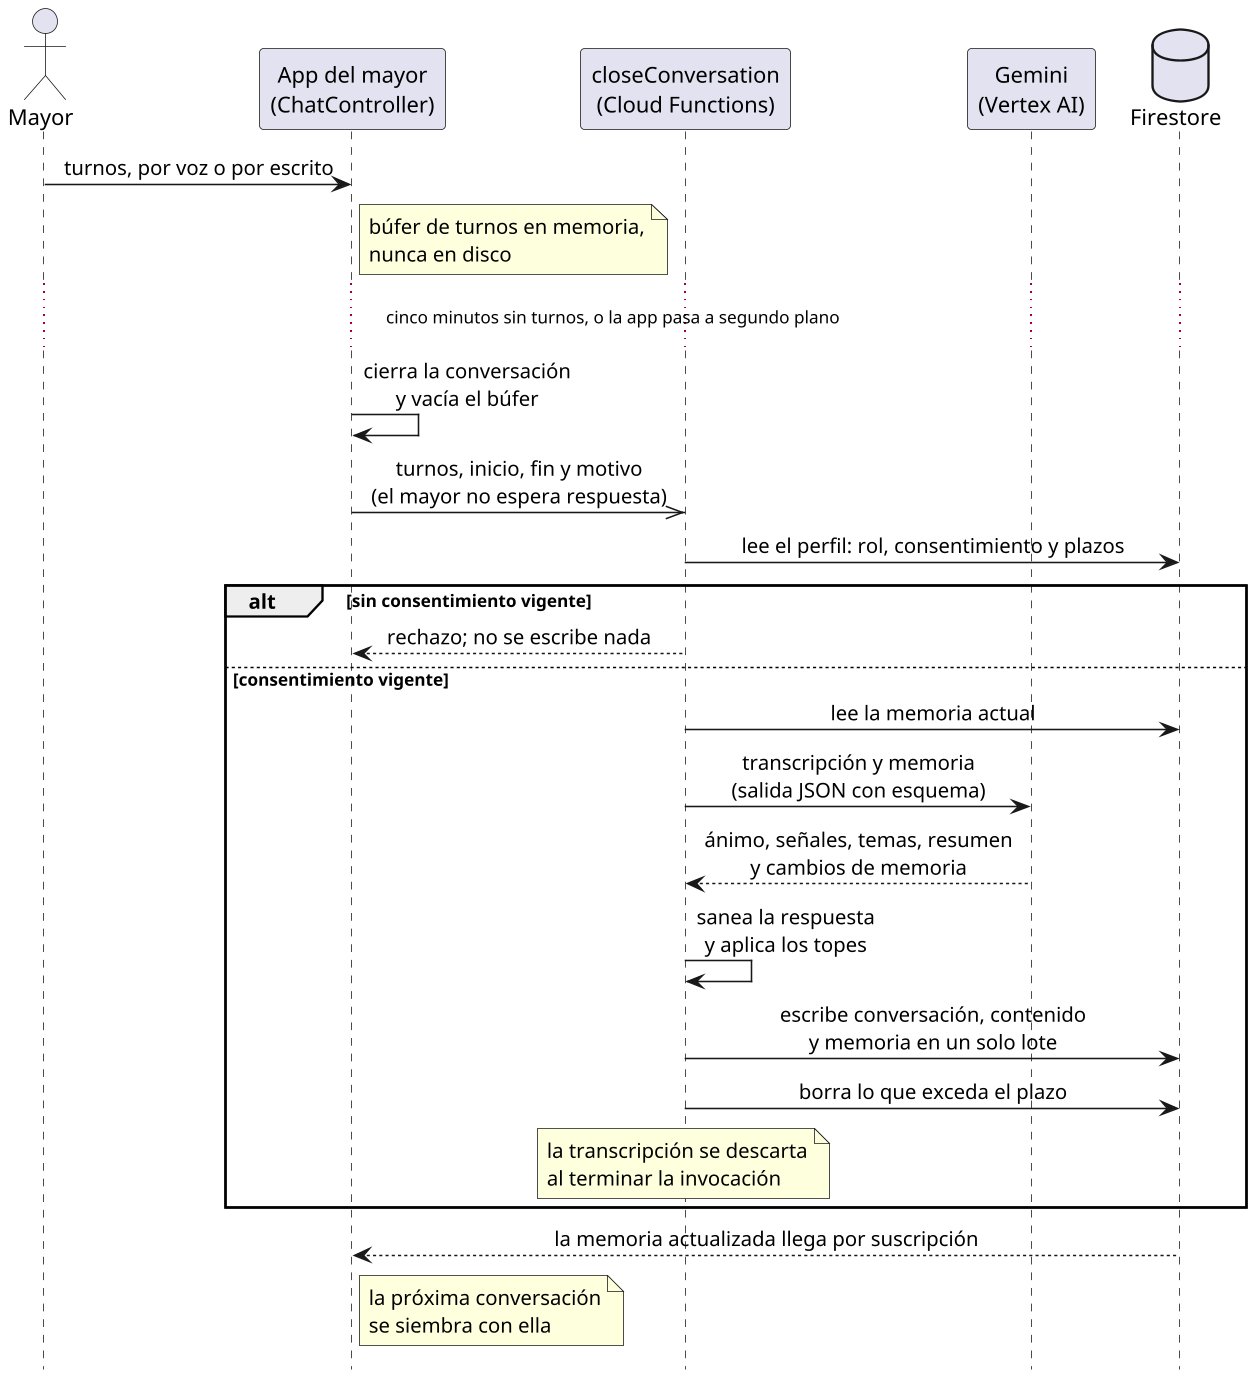
\includegraphics[width=0.85\textwidth]{imagenes/uml/secuencia_cierre.png}
    \caption{Cierre y análisis de una conversación: del búfer en memoria del teléfono a los documentos que
    se guardan, sin que la transcripción llegue a almacenarse.}
    \label{fig:secuencia-cierre}

    \vspace{2pt}
    {\footnotesize Fuente: Elaboración propia.}
\end{figure}

El valor del análisis reside en los criterios del \emph{prompt}, que se versiona y queda registrado junto a
cada resultado. El sentimiento es el del mayor y no el del diálogo, porque el asistente es cálido siempre y
evaluar la conversación entera daría «positivo» casi siempre. Las clases son las tres de RF-8, sin escalas
numéricas de valencia y activación que aparentarían una precisión que un modelo sin calibrar no tiene. Las
señales salen de una lista cerrada de seis (soledad, tristeza, preocupación, malestar físico, desorientación
y riesgo) y solo cuentan si las expresa el mayor, no si el asistente pregunta por ellas. El resumen ocupa
una o dos frases en tercera persona, sin citas literales ni diagnósticos, y nombra a otras personas por su
relación y no por su nombre. Y el \emph{prompt} advierte de que el texto procede de un reconocedor de voz,
con sus errores. Si el modelo falla, la conversación se registra igualmente como actividad, con estado de
fallo y sin reintentos, porque que el mayor hablase es un dato en sí mismo. El \autoref{lst:modelo-datos}
muestra lo que se guarda, repartido en documentos que comparten identificador; el reparto lo impone el
control de lo que ve el familiar, que se explica en el apartado~\ref{sec:privacidad}.

\begin{lstlisting}[style=Consola, caption={Lo que se guarda de cada conversación en Firestore. La transcripción no aparece en ninguno de los documentos.}, label={lst:modelo-datos}]
users/{elderId}/conversations/{id}         # "como me encuentro"
  startedAt, endedAt, elderTurns, endReason
  status:    analyzed | too_short | failed
  sentiment: positive | neutral | negative | null
  signals:   [loneliness, sadness, worry,
              physical_discomfort, confusion, risk]
  promptVersion, model, expireAt

users/{elderId}/conversationContents/{id}  # "de que hablamos"
  endedAt, topics (max. 5), summary, expireAt

users/{elderId}/memory/profile             # lo que recuerda
  facts (max. 30), recent (3 ultimos resumenes), updatedAt
\end{lstlisting}

Dos límites se declaran junto al diseño. El primero es que las etiquetas de un modelo de lenguaje no están
validadas clínicamente, de modo que se presentan como orientación y nunca como diagnóstico. El segundo, que
la señal de riesgo no convierte la aplicación en un sistema de alertas: el familiar la ve cuando abre el
panel. La respuesta a una situación de crisis corresponde al chat en vivo, cuya instrucción de sistema
incluye una regla explícita: responder con calma y sin quitarle importancia, animar a hablarlo con alguien de
confianza y recordar el 024, la línea de atención a la conducta suicida, y el 112.

\subsection{La memoria del mayor}

La API de Gemini no recuerda nada entre llamadas: la sesión del paquete de cliente es una lista de mensajes
en la memoria del teléfono que se reenvía entera en cada turno y desaparece con ella. Cualquier memoria entre
conversaciones tiene que guardarse fuera y volver a entregarse al modelo. El plan inicial de HU-5 lo
resolvía en tiempo real, con una función que el modelo invocaría a mitad de conversación para guardar cada
dato, y se descartó por una cuestión de momento oportuno (ADR-0032): la memoria solo se \emph{usa} al empezar
la conversación siguiente, así que basta con \emph{aprenderla} al terminar la anterior. Aprenderla ahí es
además gratis, porque la llamada del análisis ya lee la transcripción entera, y no añade latencia a lo único
que el mayor percibe, la respuesta en vivo.

La misma llamada del cierre devuelve, por tanto, los \textbf{cambios} de la memoria y no un perfil reescrito:
altas o correcciones por clave y claves que olvidar. Una lista de cambios explícitos se puede auditar,
mientras que un perfil regenerado entero puede perder datos sin que nadie lo note. La función los aplica con
topes estrictos, treinta datos en total y diez cambios por conversación con claves saneadas, y los guarda en
un documento propio junto a los resúmenes de las tres últimas conversaciones. El \emph{prompt} excluye
cualquier dato de salud, limita los datos de terceros a su nombre y su relación, y trata como borrado lo que
el mayor pide olvidar.

Al empezar cada conversación, la sesión del modelo se siembra con un bloque adicional en su instrucción de
sistema, «Lo que sabes de\ldots» y «De vuestras últimas conversaciones», acompañado de la indicación de
usarlo con naturalidad, no recitarlo y no decir que se tienen notas; si la memoria está vacía, el bloque no
aparece. La memoria llega al controlador del chat por suscripción y sin reconstruirlo, y una actualización
nunca reinicia una conversación en curso: se aplica en la siguiente. Solo el nombre se sigue aprendiendo en
vivo, mediante la función que el modelo invoca al oírlo, porque hace falta en la misma conversación. Es la
materialización del «RAG parcial» que anunciaba ADR-0002, sin infraestructura de búsqueda vectorial, que
sería desproporcionada para treinta datos. Por diseño, la memoria va una conversación por detrás: lo que se
cuenta hoy se recuerda a partir de la siguiente.

\subsection{El seguimiento del bienestar: el panel del familiar y «Mi semana»}
\label{sec:bienestar}

El diseño inicial pensaba el análisis solo para el familiar, lo que al mayor independiente no le aportaba
nada y al vinculado lo dejaba como objeto de seguimiento y no como destinatario de lo que se dice de él.
ADR-0033 lo invirtió sin coste de arquitectura: \textbf{los mismos datos, dos pantallas}. Los modelos de
lectura del análisis y la agregación semanal viven en \code{core/}, y la agregación es una función pura con
pruebas, \code{summarizeWeek}, que calcula los días con conversación, el ánimo predominante, los temas más
repetidos, los temas de las conversaciones con preocupación y el recuento de señales. Si cada pantalla
calculara por su cuenta, el mayor y su familiar acabarían viendo números distintos. Lo único que difiere
entre los dos lados es la presentación, y ahí difiere todo.

El \textbf{panel del familiar} ordena sus secciones por fiabilidad: primero la actividad, que no depende de
ningún modelo (cuándo habló por última vez, cuántos días y cuánto tiempo), y después las señales, el ánimo,
los temas, la lista de conversaciones con su detalle y lo que el asistente recuerda. Todo lo que estima el
modelo lleva el aviso «Orientativo: lo estima un modelo de IA a partir de lo que dice. No es un
diagnóstico». Si alguna conversación de la semana registró la señal de riesgo, el panel lo indica arriba y en
rojo, con el 112 y el 024, que atiende también a familiares. Y si el mayor ha restringido lo que comparte, el
panel lo explica en lugar de mostrar un error de permisos.

\textbf{«Mi semana»} es la pantalla del mayor, y sus reglas son las de su interfaz: frases y no gráficas, en
segunda persona y en tono de refuerzo, con un botón «Escuchar» que las lee en voz alta («Esta semana hemos
hablado 4 días», «La mayoría de las veces te he notado bien»). Una fila de siete días marca cuándo se
habló y no cómo se encontraba cada día, porque busca reforzar y no evaluar. Las señales de soledad, tristeza
o riesgo no se nombran nunca; de ellas solo aflora, suavizado, «lo que más te ha rondado la cabeza». En caso
de empate entre ánimos la agregación devuelve neutro: ante la duda, no se afirma ni que estuvo bien ni que
estuvo mal. La pantalla indica, por último, qué parte de su análisis ve su familiar, con acceso directo para
cambiarlo, de modo que «Mi semana» es también la ventana del mayor a lo que se guarda de él. El acceso aparece
en la pantalla principal para todo mayor con el consentimiento activo y al menos una conversación analizada,
sea independiente o vinculado.
% **note:** añadir capturas de «Mi semana» y del panel de bienestar del familiar cuando se hayan verificado
% en dispositivo (figura a dos paneles con subfigure, como la fig:mockups).

\section{Privacidad desde el diseño: el consentimiento informado}
\label{sec:privacidad}

De todo lo que hace el sistema, analizar las conversaciones de una persona mayor es lo más delicado, y es
también lo que más lo separa de los compañeros conversacionales revisados en el
capítulo~\ref{cap:marco-teorico}, uno de los cuales fue sancionado precisamente por carecer de base jurídica
para tratar datos. Inferir el estado de ánimo o registrar molestias físicas puede revelar datos relativos a
la salud, una categoría especial cuyo tratamiento el RGPD prohíbe salvo excepciones (art.~9.1), y la única
realista para esta aplicación es el consentimiento explícito del interesado (art.~9.2.a)
\citep{RGPD2016}. Este apartado explica cómo se ha diseñado ese consentimiento (ADR-0030), cómo se hace
cumplir (ADR-0031) y cómo se gobierna el plazo de conservación (ADR-0034). Conviene advertir de entrada su
alcance: es un diseño conforme a los principios del Reglamento, no un dictamen jurídico.

\subsection{Quién consiente, cuándo y cómo}

Un aviso no es consentimiento. El Reglamento lo define como una manifestación de voluntad libre, específica,
informada e inequívoca, mediante una declaración o una clara acción afirmativa (art.~4.11), y precisa que el
silencio, las casillas ya marcadas o la inacción no lo constituyen (considerando~32). Hace falta, por tanto,
un gesto, y el diseño solo decide cuál. Para esta población es una pantalla propia con una sola pregunta,
«¿Quieres que guarde un resumen de nuestras conversaciones?», y dos botones del mismo tamaño, «Sí, quiero» y
«Ahora no», de modo que negarse cuesta exactamente lo mismo que aceptar. No es una casilla, porque una
casilla de tamaño convencional incumpliría el área táctil mínima de RNF-2. Un botón «Escuchar» lee en voz alta
la pregunta y su explicación, y «Saber más» abre la versión completa del texto.

Consiente siempre el mayor, en su propio dispositivo. Durante el diseño se planteó que, en el modo
vinculado, pudiera consentir el familiar, y se descartó por dos motivos. El jurídico: en esta aplicación,
«vinculado» significa que al mayor le ayudan con la tecnología, no que exista una medida de apoyo que
convierta al familiar en su representante, de modo que su consentimiento no sería válido. Y el ético: sería
paternalista. La solución separa dos papeles que aquella propuesta mezclaba, \textbf{ayudar a decidir}, que
corresponde al familiar, y \textbf{decidir}, que corresponde al mayor. La pregunta aparece una sola vez y en
el momento más temprano posible: justo después de elegir el modo independiente o justo después de
completarse la vinculación, un momento que suele ser presencial, porque el familiar lee el código en la
pantalla del mayor y puede explicarle la pregunta en persona. Se implementa como un paso del enrutador, y
«Ahora no» también se registra, para no volver a preguntar.

El texto está en lenguaje llano y se ofrece en dos capas, una breve en la pregunta y otra completa en «Saber
más», en la línea de los artículos~12 y~13. Explica por separado qué se guarda (un resumen breve de cada
conversación y cómo se ha sentido, nunca lo que dice palabra por palabra), qué se recuerda (lo que cuenta de
su familia o de sus gustos, nunca nada de su salud), cómo se hace (lo hablado se envía a los servidores de
Google, que lo analizan y no lo guardan), quién lo ve (su familiar, por su nombre, o solo él), cuánto tiempo
se conserva y cómo puede retirarlo. El texto está versionado, y la versión leída se registra con la
respuesta. Un único consentimiento cubre el análisis y la memoria, porque ambos sirven al propio mayor; lo
que ve el familiar es una decisión aparte. Y nada se trata hasta el «sí»: el consentimiento está desactivado
por defecto, que es la protección de datos por defecto del artículo~25.2.

\subsection{Cómo se hace cumplir}

Un consentimiento que solo respeta la interfaz no protege nada, porque el familiar tiene sesión propia y
podría leer cuanto las reglas le permitan, con esta aplicación o con otra. Por eso las tres garantías
centrales se imponen en el servidor.

La primera es la \textbf{prueba del consentimiento}. El responsable debe poder demostrar que el interesado
consintió (art.~7.1), y una hora tomada del dispositivo no demuestra nada. El registro del consentimiento,
con la respuesta, la hora y la versión del texto leído, solo lo escribe \code{setConversationConsent}, con la
hora del servidor; las reglas impiden que lo escriba cualquier cliente, incluido el propio mayor, y que un
documento nazca con un consentimiento de serie. La función toma además la identidad de la sesión, de modo que
un familiar no puede consentir por su mayor ni siquiera llamándola directamente.

La segunda es que \textbf{sin consentimiento no se analiza nada}. El cliente no envía la conversación si no
lo hay, pero la garantía real es que \code{closeConversation} lo vuelve a comprobar y, si no está vigente,
rechaza la petición sin escribir nada.

La tercera es \textbf{qué ve el familiar} (ADR-0031). El mayor elige entre tres niveles con nombre: «Nada»;
«Cómo me encuentro», que incluye la actividad, el ánimo y las señales; y «Cómo me encuentro y de qué
hablamos», que añade los temas, los resúmenes y la memoria. Solo el mayor puede escribir ese nivel. Hacerlo
cumplir tropieza con una limitación ya conocida de Firestore, la de que las reglas no pueden filtrar campos,
porque leer un documento es leerlo entero. La solución está en el almacenamiento: cada conversación se
reparte en dos documentos, y las reglas conceden la lectura de cada colección según el nivel. El
\autoref{lst:reglas} muestra la función que lo decide.

\begin{lstlisting}[float=tbp, caption={Regla de lectura del familiar sobre el análisis del mayor (extracto de \texttt{firestore.rules}).}, label={lst:reglas}]
function companionMayRead(elderId, levels) {
  let elder = get(/databases/$(database)/documents/users/$(elderId)).data;
  return isSignedIn()
    && elder.get('linkedCompanionId', null) == request.auth.uid
    && elder.get('conversationConsent', {}).get('granted', false) == true
    && elder.get('companionSharing', 'none') in levels;
}

match /users/{userId} {
  match /conversations/{id} {             // como me encuentro
    allow read: if isOwner(userId)
      || companionMayRead(userId, ['wellbeing', 'full']);
    allow write: if false;                // solo el servidor
  }
  match /conversationContents/{id} {      // de que hablamos
    allow read: if isOwner(userId)
      || companionMayRead(userId, ['full']);
    allow write: if false;
  }
}
\end{lstlisting}

La condición se evalúa al leer y no se copia al escribir, de modo que bajar el nivel oculta al instante
también todo el historial. Las pruebas contra el emulador verifican cada caso; por ejemplo, un familiar con
nivel «Cómo me encuentro» que intenta leer los resúmenes es rechazado. Queda un coste ético asumido y
declarado: las señales, también la de riesgo, pertenecen al nivel intermedio, y si el mayor elige «Nada» su
familiar no sabrá que la hubo. Prima la autonomía del mayor, coherente con que la aplicación no es un sistema
de alertas.

\subsection{Retirada, plazos y borrado}

Retirar el consentimiento debe ser tan fácil como darlo (art.~7.3). En Ajustes, la fila «Guardar mis
conversaciones» permite hacerlo con un toque y una confirmación que muestra la fecha en que se borrará lo
guardado. La retirada tiene efecto inmediato sobre el tratamiento: se detiene el análisis, la memoria deja
de inyectarse y el familiar pierde el acceso, porque sus reglas de lectura exigen el consentimiento vigente
además del nivel. Lo ya guardado, en cambio, no se borra al instante. Queda congelado durante un periodo de
gracia igual a la mitad del plazo de conservación vigente, cuarenta y cinco días con el plazo por omisión,
durante el que nadie lo trata ni lo lee salvo el propio mayor; si vuelve a consentir antes, lo recupera, y si
no, se borra. El motivo es proteger al mayor de una retirada accidental: en esta población, un toque
equivocado no debería costar meses de historia. La tensión con el artículo~17.1.b, que pide suprimir los
datos sin dilación indebida cuando se retira el consentimiento, se declara en lugar de esconderse: se
defiende por su finalidad y porque durante el periodo los datos no se tratan, y una opción «Borrarlo ya» la
eliminaría del todo.

El borrado no exige ninguna tarea programada. Cada documento del análisis lleva una fecha de caducidad, y
una política de caducidad (TTL) de Firestore lo elimina al vencer, normalmente dentro de las veinticuatro
horas siguientes \citep{FirestoreTTL}. Al retirar el consentimiento, la función adelanta esa fecha en cada
documento a la más temprana entre su caducidad normal y el final del periodo de gracia, de modo que retirarlo
nunca alarga la vida de un dato; al volver a consentir, la restaura.

Los plazos, por último, son configurables (ADR-0034): el tiempo sin turnos que cierra una conversación (2, 5,
10 o 15~minutos) y el plazo de conservación (30, 60, 90 o 180~días, con 90 por omisión). Siguen el reparto
de la revelación progresiva: los fija el propio mayor si es independiente y su familiar, desde el panel, si
está vinculado. Como el segundo afecta a datos personales, lleva un tope que ningún papel puede superar: el
servidor lo acota entre 30 y 180~días diga lo que diga el documento, y en cada cierre borra lo que haya
quedado fuera del plazo vigente, de modo que acortarlo borra de verdad sin esperar a la caducidad de lo
antiguo. Queda una tensión declarada: el mayor vinculado consiente con el plazo vigente en ese momento y su
familiar puede alargarlo después hasta seis meses; el texto del consentimiento lo advierte y la pantalla de
detalle muestra siempre el valor actual.

\subsection{Correspondencia con el RGPD y límites}

La \autoref{tab:rgpd} resume cómo se realizan en el sistema las obligaciones del Reglamento que afectan al
tratamiento de las conversaciones.

\begin{table}[htbp]
    \centering
    \small
    \begin{tabularx}{\textwidth}{@{}>{\RaggedRight\arraybackslash}p{0.36\textwidth} >{\RaggedRight\arraybackslash}X@{}}
        \toprule
        \textbf{Obligación del RGPD} & \textbf{Realización en Quiet Companion} \\
        \midrule
        Base de licitud para datos de salud: consentimiento explícito (arts.~6.1.a y 9.2.a)
            & Pantalla propia con un gesto afirmativo del mayor; el familiar no puede consentir por él \\
        Consentimiento inequívoco (art.~4.11, considerando~32)
            & Dos botones del mismo tamaño; ni silencio ni casillas premarcadas \\
        Información clara y accesible (arts.~12 y 13)
            & Texto llano y versionado, en dos capas y con lectura en voz alta \\
        Demostrar el consentimiento (art.~7.1)
            & Registro escrito solo por el servidor, con su hora y la versión del texto \\
        Retirarlo tan fácilmente como se dio (art.~7.3)
            & Una fila en Ajustes, un toque y una confirmación \\
        Minimización de datos (art.~5.1.c)
            & La transcripción no se almacena; sin texto por debajo de tres turnos; un solo análisis \\
        Limitación del plazo de conservación (art.~5.1.e)
            & Caducidad automática (TTL); plazo de 30 a 180~días acotado por el servidor \\
        Protección de datos desde el diseño y por defecto (art.~25)
            & Desactivado por defecto; niveles de compartición impuestos por las reglas \\
        Derecho de acceso (art.~15)
            & «Mi semana» muestra al mayor lo que se guarda de él y quién lo ve \\
        Derecho de supresión (art.~17.1.b)
            & Borrado al final del periodo de gracia tras la retirada \\
        Seguridad del tratamiento (art.~32)
            & Reglas verificadas contra el emulador; registros sin texto de las conversaciones \\
        \bottomrule
    \end{tabularx}
    \caption{Correspondencia entre las obligaciones del RGPD y su realización en el sistema.}
    \label{tab:rgpd}

    \vspace{2pt}
    {\footnotesize Fuente: Elaboración propia a partir del Reglamento (UE) 2016/679.}
\end{table}

El diseño tiene límites que deben constar. Un despliegue real con personas mayores y datos de salud exigiría
una evaluación de impacto relativa a la protección de datos (art.~35), que queda como trabajo futuro. Un
revisor estricto podría pedir separar el consentimiento del análisis del de la memoria, hoy unificados porque
ambos benefician al mayor. Y lo hablado sale del dispositivo hacia Google en dos momentos: en cada turno de
la conversación en vivo y en su análisis al cierre. En ninguno de los dos puede el proveedor usarlo para
mejorar sus modelos: el análisis se sirve desde Vertex AI en una región europea, cuyas condiciones excluyen
entrenar con los datos del cliente sin su permiso \citep{VertexDataGovernance}, y las condiciones de la API
de Gemini extienden esa misma exclusión a la cuota gratuita para los usuarios del Espacio Económico Europeo,
con una retención limitada de las peticiones para detectar abusos \citep{GeminiTerms}. Ese tratamiento por
un tercero es el que el texto del consentimiento hace explícito.

\section{Conversación por escrito}
\label{sec:teclado}

La voz es el canal principal del mayor, pero no siempre el adecuado: en una sala de espera, de noche con
alguien durmiendo, con ronquera o con una dificultad del habla, o simplemente cuando el reconocedor no le
entiende. Ese último caso no es teórico, porque la escucha por turnos ha sido la pieza más difícil de
estabilizar del proyecto. La pantalla principal mostraba además, desde su rediseño, un botón «¿Teclado?» que
no hacía nada, y para este usuario un botón que no responde es un fallo tan grave como un callejón sin
salida. HU-8 lo convirtió en funcionalidad (ADR-0035).

El coste de añadir el canal fue casi solo de presentación, porque la arquitectura ya separaba la entrada de
la conversación: el método del controlador que envía un turno no sabe de dónde viene el texto. Un turno
escrito sigue por tanto \textbf{el mismo camino} que uno hablado, con la misma sesión del modelo, el mismo
búfer en memoria y la misma frontera de conversación, de modo que cuenta para el mínimo de tres turnos y
llega al análisis al cierre sin tocar el servidor. No lleva marca de canal, porque el análisis trata de lo
que dice el mayor y no de cómo lo dice.

La decisión que de verdad había que tomar era otra: si la aplicación habla cuando el mayor no habla. La
respuesta es que no, salvo que lo pida. La respuesta a un turno escrito se muestra sin leerse, porque el
motivo más común para escribir es estar donde no se quiere que el teléfono hable, y un botón «Escuchar», que
mientras suena pasa a «Parar», devuelve la voz a quien escribe por una dificultad del habla pero necesita oír
la respuesta. El turno hablado no cambia. Pulsar «¿Teclado?» sustituye el micrófono por un campo de texto,
con la letra escalada por la preferencia del mayor, y un botón «Enviar» de $80\times80$ píxeles lógicos; el
campo toma el foco al aparecer, de modo que el teclado del sistema se abre sin otro toque, y el mismo botón
pasa a decir «¿Hablar?» para volver. Si el envío falla, el texto vuelve al campo para no obligar a escribirlo
de nuevo.

Dos detalles de implementación merecen constar porque resuelven problemas que no se ven en la interfaz. El
modo vive en el estado del controlador y no en el \emph{widget}, de modo que sobrevive a ir a Ajustes o a
Emergencia y volver, y el controlador puede actuar al cambiarlo: pasar al teclado con el micrófono abierto
\textbf{descarta} lo que se estaba oyendo en lugar de enviar un texto que el mayor no ha confirmado. Y como
una voz cortada termina tarde, cuando ya ha empezado otra cosa, cada turno, escucha o lectura toma un número
de orden, y la vuelta a reposo tras hablar solo se aplica si lo que la lanzó sigue siendo lo último. Sin ese
control, una respuesta cortada por un turno escrito devolvía la pantalla a reposo con el turno nuevo en curso
y permitía enviar un segundo mensaje simultáneo a la misma sesión del modelo. El predicado que decide si se
admite un turno escrito está en un solo sitio, el estado del chat, y lo consultan por igual la pantalla y el
controlador.

\section{Cronología del desarrollo}
\label{sec:cronologia}

El plan de hitos se documenta en el capítulo~\ref{cap:metodologia}; lo que sigue es cómo se construyó, fase
a fase, y qué desviaciones se produjeron. La \autoref{tab:fases} resume las fases y su correspondencia con
los hitos del plan.

\begin{table}[htbp]
    \centering
    \small
    \begin{tabularx}{\textwidth}{@{}>{\RaggedRight\arraybackslash}p{0.27\textwidth} l l >{\RaggedRight\arraybackslash}X@{}}
        \toprule
        \textbf{Fase} & \textbf{Periodo} & \textbf{Hitos} & \textbf{Qué entregó} \\
        \midrule
        0. Arranque                        & Marzo      & ---    & Repositorio y descripción del proyecto \\
        1. Prototipo y \emph{stack}        & Marzo      & M1, M2 & Voz de extremo a extremo y elección del \emph{stack} (ADR-0001 a 0005) \\
        2. Onboarding y panel remoto       & Abril      & M1, M3 & Onboarding dual, emparejamiento y panel del familiar (ADR-0006 a 0010) \\
        3. Estabilización                  & Mayo--jul. & M4     & Navegación, inyección de dependencias, emergencia, ajustes y primera suite de pruebas \\
        4. Voz en la nube y endurecimiento & Jul.--sep. & M5     & Voz Chirp~3:~HD, escucha por turnos, reglas verificadas y vinculación en el servidor (ADR-0017 a 0026) \\
        5. Privacidad y bienestar          & Septiembre & M6, M7 & Consentimiento, análisis al cierre, memoria, panel y «Mi semana» (ADR-0027 a 0034) \\
        6. Conversación por escrito        & Octubre    & M8     & Modo teclado y correcciones de la prueba en dispositivo (ADR-0035 y 0036) \\
        \bottomrule
    \end{tabularx}
    \caption{Fases del desarrollo y su correspondencia con los hitos (2026).}
    \label{tab:fases}
\end{table}

Tres rasgos de esa secuencia merecen comentario. El proyecto arrancó demostrando lo más arriesgado primero,
que la cadena de reconocimiento, generación y síntesis de voz funcionaba de extremo a extremo, antes de
construir nada a su alrededor. La fase~4 cambió la naturaleza del sistema: la aplicación dejó de ser un
cliente que habla con servicios ajenos y pasó a tener servidor propio, primero para la voz y después para la
seguridad. Y la fase~5 se ordenó por dependencias de privacidad y no de funcionalidad: el panel en tiempo
real y el consentimiento precedieron a cualquier análisis, porque ningún dato de una conversación podía
tratarse antes de que existiera el permiso que lo autoriza, ni guardarse en un documento que el panel del
familiar pudiera reescribir.

Dos observaciones más deben hacerse explícitas. La primera es que \textbf{la velocidad no fue uniforme}: el
desarrollo procedió en incrementos por Historia de Usuario ejecutados en sesiones concentradas, en paralelo
a un empleo a tiempo completo, y la estabilización se alargó al coincidir con el periodo de exámenes. Esa
cadencia a ráfagas es una consecuencia de las condiciones del proyecto, no un defecto de método: cada ráfaga
cerró un incremento coherente y dejó el código compilable y estabilizado.

La segunda es que \textbf{el bucle de revisión es visible en el propio proceso}, y ésa es la evidencia más
valiosa que ofrece. El hito 2.5 de HU-4 no estaba planificado: existe porque una revisión de arquitectura,
al auditar el hito anterior, detectó dos violaciones de reglas preexistentes (la instanciación directa de servicios y el acoplamiento horizontal del \emph{dashboard}), que se corrigieron a mitad del hito. El
mismo patrón se repite con el defecto de re-login del familiar durante la estabilización; con las reglas de
seguridad de la fase~4, cuyos primeros veintinueve casos de prueba se escribieron \emph{incluyendo los
huecos} y fueron los que hicieron visible que la vinculación desde el cliente obligaba a dejar el directorio
de usuarios enumerable; con el panel que revertía en silencio los cambios del mayor, descubierto al diseñar
HU-5 y HU-6 (ADR-0027); y con la primera prueba completa en dispositivo, que destapó la palabra perdida de la
escucha (ADR-0036). Un proceso sin tropiezos aparentes habría sido menos informativo: revisión, hallazgo y
refactorización es lo que se pretende demostrar.

\section{Cierre del capítulo}

El sistema descrito en este capítulo cumple los requisitos comprometidos con una excepción declarada y un
conjunto acotado de deuda conocida, y conviene enumerarlas juntas.

En cuanto a la \textbf{verificación}, el árbol de código pasa el análisis estático sin advertencias (RNF-13)
y cuenta con tres suites complementarias: unos doscientos casos en Dart, que cubren los modelos, el
enrutador, los controladores del chat y del panel, la escucha por turnos, las pantallas del mayor, la
agregación semanal y la síntesis de voz; cuarenta y ocho casos de reglas de seguridad contra el emulador de
Firestore; y cuarenta y cuatro casos sobre la lógica pura de las funciones del servidor. La verificación en
dispositivo es completa para el MVP y está en curso para los incrementos posteriores: la primera prueba
completa de una conversación en el móvil ya se ha hecho y sus hallazgos se han corregido (ADR-0036), pero el
recorrido de HU-5 a HU-8 quedaba pendiente al redactar esta memoria, y no existe todavía integración
continua que ejecute las tres suites juntas.
% **note:** fijar las cifras exactas de las suites (Dart, reglas y funciones) cuando se ejecuten todas en
% verde antes de la entrega, y actualizar el estado de la verificación en dispositivo de HU-5 a HU-8.

El \textbf{compromiso abierto} es de seguridad: la clave de Gemini de la conversación en vivo reside en el
cliente, de modo que RNF-8 se cumple solo en parte (ADR-0014). Varios compromisos que este capítulo mantuvo
abiertos durante el desarrollo se \textbf{cerraron}, en cambio, antes de su final: RNF-9, con la vinculación
en el servidor y unas reglas verificadas (ADR-0024 a ADR-0026); CU-05, con las escalas locales de
accesibilidad (ADR-0021); el modelo de consentimiento que bloqueaba HU-5 (ADR-0030); y el botón «¿Teclado?»,
durante meses una afordancia inerte y hoy la conversación por escrito (ADR-0035). La \textbf{deuda menor}
incluye el camino de desbloqueo redundante citado, la ausencia de reintento ante colisión de códigos de
vinculación (riesgo asumido con unas 923\,000 combinaciones posibles) y el color del estado
\emph{Pensando}, que no alcanza el contraste no textual (\autoref{sec:color}).

Ninguno de estos puntos invalida el resultado: la aplicación conversa por voz o por escrito, recuerda lo que
el mayor le cuenta, informa de cómo se encuentra a quien él autoriza, se configura en remoto, llama a
emergencias y se adapta a las capacidades de quien la usa, sin guardar nunca lo que dice palabra por palabra.
Pero delimitan con precisión dónde termina lo construido y empieza lo decidido. Esa frontera, y las líneas de
trabajo que arrancan de ella, se desarrollan en el \autoref{cap:desarrollo-futuro}.
